\documentclass[12pt, a4paper]{report}
\usepackage[utf8]{inputenc}
\usepackage{graphicx}
\usepackage{amsmath}
\usepackage{amssymb}
\usepackage{booktabs}
\usepackage{longtable}
\usepackage{tabularx}
\usepackage{array}
\usepackage{hyperref}
\usepackage{geometry}
\usepackage{float}
\geometry{a4paper, left=1.5in, right=1in, top=1in, bottom=1in}
\usepackage{setspace}
\onehalfspacing
\usepackage{titlesec}
\titleformat{\chapter}[display]
  {\normalfont\huge\bfseries\centering}{\chaptertitlename\ \thechapter}{10pt}{\Huge}
\titlespacing*{\chapter}{0pt}{-30pt}{20pt}

\begin{document}

\begin{titlepage}
    \centering
    \vspace*{1in}
    {\LARGE \textbf{AI-Powered Supply Chain Intelligence Platform}}\par
    \vspace{1.5in}
    {\large Submitted in partial fulfillment of the requirements for the degree of}\par
    \vspace{0.2in}
    {\Large \textbf{Master of Data Science (Online)}}\par
    \vspace{1in}
    {\large by}\par
    \vspace{0.2in}
    {\Large \textbf{[Learner Name]}}\par
    {\large \textbf{[Learner Reg. No]}}\par
    \vspace{1in}
    {\large Under the guidance of \textbf{[Guide Name]}}\par
    \vspace{1in}
    {\large \textbf{June 2026}}\par
    {\large \textbf{VIT Online Learning Program}}\par
\end{titlepage}

\pagenumbering{roman}

\chapter*{DECLARATION}
\addcontentsline{toc}{chapter}{DECLARATION}
I, [Learner Name], with register number [Learner Reg. No] hereby declare that the project report entitled ``AI-Powered Supply Chain Intelligence Platform'' submitted by me to M.Sc., Data Science VIT Online learning program, Vellore, in partial fulfilment of the requirement for the award of the degree of Master of Data Science is a Bonafide work carried out by me under the supervision of Prof. [Guide Name], [Designation], [Department], [School], Vellore Institute of Technology, Vellore - 632 014.

I further declare that the work reported in this project has not been submitted and will not be submitted, either in part or in full, for the award of any other degree or diploma in this institute or any other Institute or University.

\vspace{0.5in}
\noindent Place: VIT VELLORE \newline
Date: [Date] \hfill \textbf{[LEARNER NAME]} \newline
\null \hfill Signature of the Candidate

\chapter*{CERTIFICATE}
\addcontentsline{toc}{chapter}{CERTIFICATE}
This is to certify that the project work entitled ``AI-Powered Supply Chain Intelligence Platform'' submitted by [Learner Name] with registration number [Learner Reg. No], to VIT Vellore, in partial fulfilment of the requirement for the award of the degree of Master of Data Science, is a bona fide work carried out by him/her under my supervision. The project fulfils the requirements as per VIT Vellore regulations and, in my opinion, meets the necessary standards for submission. The contents of this report have not been submitted and will not be submitted either in part or in full, for the award of any other degree or diploma in this Institute or any other Institute or University.

\vspace{0.5in}
\noindent Place: VIT VELLORE \newline
Date: \newline

\vspace{0.5in}
\noindent Guide Name \& Signature \newline
Examiner 1: HOD Online M.Sc. DS \newline
Examiner 2: Director, VITOL

\chapter*{ACKNOWLEDGEMENT}
\addcontentsline{toc}{chapter}{ACKNOWLEDGEMENT}
At the outset, I thank the Almighty God for His blessings for granting me the knowledge and right aptitude to successfully complete my project work.

I would like to express my special gratitude and thanks to my guide [Guide Name], [Designation], [School], whose esteemed guidance and immense support encouraged me to complete the project successfully.

My sincere thanks to Honourable Chancellor, Dr. G. VISWANATHAN; esteemed Vice-Presidents; respected Vice Chancellor, Dr. V. S. KANCHANA BHAASKARAN of this prestigious VIT, Vellore, for providing me an excellent world-class academic environment and facilities for pursuing my online M.Sc. Data Science Program.

My sincere gratitude lies to the Director, Dr. RHYMEND UTHARIARAJ VITOL, and the Head of the Department, online M.Sc. Data Science, VITOL, Prof. Sri Rama Vara Prasad Bhuvanagiri, for providing me with an opportunity to do my project work at VIT, Vellore.

I also thank all the faculty members of the VITOL, Department of Mathematics and the faculty of other Departments of the VIT, as well as the non-teaching staff, for giving me the courage and strength that I needed to achieve my goals.

My special thanks to my friends for their timely help and suggestions rendered for the successful completion of this project.

This acknowledgement would be incomplete without expressing my whole-hearted thanks to my parents for their continuous support and guidance in all walks of my life.

\vspace{0.5in}
\noindent \textbf{[LEARNER NAME]}

\chapter*{ABSTRACT}
\addcontentsline{toc}{chapter}{ABSTRACT}
This thesis presents \textbf{ChainPilot AI}, a comprehensive, AI-powered, multi-domain supply chain intelligence platform that bridges the gap between isolated data science research and real-world enterprise deployment. The platform integrates six advanced predictive and analytical algorithms---Auto-ARIMA, Random Forest, XGBoost with Optuna Bayesian optimization, PyTorch Long Short-Term Memory (LSTM) networks, PyTorch Gated Recurrent Units (GRU), and Isolation Forest anomaly detection---into a unified, production-grade software architecture built with FastAPI (Python backend) and React 18 (JavaScript frontend).

To demonstrate domain independence and commercial scalability, the system was validated across four massive, real-world benchmark datasets spanning distinct business verticals: (1) M5 Forecasting Accuracy (Walmart hierarchical retail demand), (2) Rossmann Store Sales (European retail promotion forecasting), (3) DataCo Smart Supply Chain (global logistics and shipping analytics), and (4) Brazilian E-Commerce Olist (end-to-end e-commerce fulfillment and freight analysis). The architecture employs walk-forward cross-validation to prevent data leakage, SHAP-based feature importance analysis for model interpretability, and a Retrieval-Augmented Generation (RAG) pipeline powered by Google Gemini and FAISS vector databases to translate complex quantitative outputs into natural-language executive recommendations.

Empirical results demonstrate that Optuna-tuned XGBoost and PyTorch LSTM architectures consistently outperform traditional statistical methods (Auto-ARIMA) across all four domains, while the Isolation Forest algorithm successfully detects multivariate supply chain anomalies that standard univariate monitoring would miss. The web application provides interactive Chart.js visualizations, dynamic KPI dashboards, and a conversational AI assistant, proving that state-of-the-art predictive analytics can be deployed as an intuitive, real-time Software-as-a-Service (SaaS) solution.

\vspace{0.2in}
\noindent \textbf{Keywords:} Supply Chain Management, Deep Learning, LSTM, XGBoost, Optuna, Anomaly Detection, Retrieval-Augmented Generation, FastAPI, React, FAISS, Demand Forecasting, PyTorch

\tableofcontents
\listoffigures
\listoftables

\clearpage
\pagenumbering{arabic}

\chapter{INTRODUCTION}

\subsection{1.1 Background and Motivation}

The global supply chain landscape has undergone a fundamental transformation in the past decade. The convergence of globalization, e-commerce expansion, pandemic-induced disruptions (COVID-19), and escalating consumer expectations for rapid delivery has exposed the critical fragility of traditional supply chain management systems. According to a 2023 McKinsey Global Institute report, companies that adopt AI-driven supply chain management can reduce logistics costs by 15\%, cut inventory levels by 35\%, and improve service levels by 65\% compared to organizations relying on legacy spreadsheet-based planning.

Traditional supply chain planning relies heavily on deterministic methods: static safety-stock calculations, manual reorder-point formulas, and basic moving-average demand estimates. These approaches assume that supply chain dynamics are linear, stationary, and predictable. However, real-world supply chains are inherently non-linear, non-stationary, and subject to sudden, unpredictable disruptions -- from factory shutdowns and port congestions to sudden demand surges driven by viral social media trends or seasonal promotions.

The emergence of advanced Machine Learning (ML) and Deep Learning (DL) architectures offers a paradigm shift. Unlike rule-based systems, ML algorithms such as Random Forest and Extreme Gradient Boosting (XGBoost) can learn complex, non-linear relationships between hundreds of operational variables. Furthermore, Deep Learning sequence models -- specifically Long Short-Term Memory (LSTM) networks and Gated Recurrent Units (GRU) -- can capture long-range temporal dependencies in time-series data, enabling accurate multi-step-ahead forecasting that traditional Auto-Regressive Integrated Moving Average (ARIMA) models cannot achieve.

However, a critical gap persists in both industry and academia: the vast majority of AI supply chain research remains confined to Jupyter Notebooks and static research papers. The models are trained, evaluated, and then abandoned. They are never integrated into real-time, user-facing software systems that operations managers and supply chain executives can actually use. This thesis addresses this gap directly.

\subsection{1.2 Problem Statement}

Despite the proven capabilities of machine learning and deep learning in demand forecasting and anomaly detection, the adoption of these technologies in real-world supply chain operations remains critically low. The primary barriers are:

\begin{enumerate}
\item 1. \textbf{The Deployment Gap:} Most data science research terminates at the Jupyter Notebook stage. Models are trained and evaluated in isolated environments but never deployed into production-grade software systems that non-technical stakeholders can interact with.
\end{enumerate}

\begin{enumerate}
\item 2. \textbf{Domain Specificity:} Existing AI supply chain solutions are typically hardcoded to work with a single dataset or a single business domain. A model trained on retail point-of-sale data cannot be applied to logistics freight optimization without significant re-engineering.
\end{enumerate}

\begin{enumerate}
\item 3. \textbf{Interpretability Deficit:} Complex machine learning models (particularly ensemble methods and deep neural networks) produce numerical outputs (e.g., RMSE = 12.1) that are meaningless to business executives. There is no translation layer that converts quantitative predictions into actionable, plain-language strategic recommendations.
\end{enumerate}

\begin{enumerate}
\item 4. \textbf{Anomaly Blindness:} Traditional quality-control methods rely on univariate control charts that monitor a single variable at a time. They cannot detect complex, multivariate anomalies -- such as a shipment with an unusually high cost combined with an abnormally long lead time and a suspiciously high defect rate -- that only manifest when multiple variables are analyzed simultaneously.
\end{enumerate}

\subsection{1.3 Research Objectives}

This thesis aims to design, implement, and evaluate a comprehensive, AI-powered supply chain intelligence platform named \textbf{ChainPilot AI} that addresses the four critical gaps identified above. The specific research objectives are:

\begin{enumerate}
\item 1. \textbf{Objective 1 (Forecasting):} To implement and comparatively evaluate six predictive architectures -- Auto-ARIMA, Random Forest, XGBoost (with Optuna Bayesian optimization), PyTorch LSTM, and PyTorch GRU -- for multi-step-ahead demand forecasting using walk-forward cross-validation.
\end{enumerate}

\begin{enumerate}
\item 2. \textbf{Objective 2 (Anomaly Detection):} To deploy an Isolation Forest algorithm for unsupervised, multivariate anomaly detection capable of identifying complex supply chain disruptions, fraud, and quality-control failures.
\end{enumerate}

\begin{enumerate}
\item 3. \textbf{Objective 3 (Domain Independence):} To prove the scalability and commercial viability of the platform by validating the algorithms across four completely distinct, real-world benchmark datasets spanning retail, logistics, and e-commerce industries.
\end{enumerate}

\begin{enumerate}
\item 4. \textbf{Objective 4 (Deployment):} To bridge the Jupyter-to-Production gap by engineering a full-stack web application using FastAPI (Python backend) and React 18 (JavaScript frontend) that allows non-technical users to upload data, execute the AI pipeline, and interact with results through dynamic visualizations and a conversational AI assistant.
\end{enumerate}

\begin{enumerate}
\item 5. \textbf{Objective 5 (Interpretability):} To integrate a Retrieval-Augmented Generation (RAG) pipeline using Google Gemini and FAISS vector databases that translates complex model outputs and SHAP feature importance rankings into natural-language executive strategy recommendations.
\end{enumerate}

\subsection{1.4 Research Questions}

The following research questions guide this investigation:

\begin{itemize}
\item \textbf{RQ1:} How do ensemble machine learning methods (Random Forest, XGBoost) and deep learning sequence models (LSTM, GRU) compare against traditional statistical methods (ARIMA) for supply chain demand forecasting across diverse business domains?
\end{itemize}

\begin{itemize}
\item \textbf{RQ2:} Can an unsupervised Isolation Forest algorithm effectively detect multivariate operational anomalies that standard univariate monitoring methods would miss?
\end{itemize}

\begin{itemize}
\item \textbf{RQ3:} How can Large Language Models (LLMs) be effectively constrained using Retrieval-Augmented Generation (RAG) to produce reliable, context-aware, prescriptive business recommendations from quantitative model outputs?
\end{itemize}

\begin{itemize}
\item \textbf{RQ4:} What software engineering architectures and deployment strategies are required to transition AI models from isolated research environments (Jupyter Notebooks) into scalable, real-time, user-facing enterprise web applications?
\end{itemize}

\subsection{1.5 Scope and Multi-Domain Data Sources}

To prove that the AI algorithms developed for ChainPilot AI are truly domain-independent and commercially scalable, this research validates the entire pipeline across four massive, publicly available benchmark datasets from Kaggle. Each dataset represents a fundamentally different business vertical and operational challenge:

\textbf{Table 1.1: Multi-Domain Dataset Summary}

\begin{table}[H]
\centering
\caption{Dataset - Domain - Records - Key Features - Primary Use Case}
\vspace{0.1in}
\begin{tabularx}{\textwidth}{|>{\raggedright\arraybackslash}X|>{\raggedright\arraybackslash}X|>{\raggedright\arraybackslash}X|>{\raggedright\arraybackslash}X|>{\raggedright\arraybackslash}X|}
\hline
Dataset & Domain & Records & Key Features & Primary Use Case \\ \hline
\hline
M5 Forecasting Accuracy & Retail (Walmart) & 30,490 products, ~58M data points & Hierarchical product categories, store locations, calendar events, SNAP eligibility & Hierarchical demand forecasting across massive product taxonomies \\ \hline
Rossmann Store Sales & Retail (European Drug Stores) & 1,017,209 daily records across 1,115 stores & Promotions, school/state holidays, competitor distance, store type & Promotion-driven sales forecasting with holiday seasonality \\ \hline
DataCo Smart Supply Chain & Logistics \& Manufacturing & 180,519 supply chain records & Shipping modes, delivery status, order regions, product categories, profit margins & Logistics optimization, shipping delay prediction, fraud detection \\ \hline
Brazilian E-Commerce (Olist) & E-Commerce & 99,441 orders across 8 relational tables & Freight values, delivery timestamps, customer reviews, seller locations, product dimensions & End-to-end e-commerce fulfillment analysis, freight cost optimization \\ \hline
\end{tabularx}
\end{table}

The deliberate selection of these four datasets ensures that the ChainPilot AI architecture is tested against:
\begin{itemize}
\item \textbf{Temporal complexity} (M5 and Rossmann with deep chronological histories)
\item \textbf{Spatial complexity} (DataCo with global shipping routes and Olist with Brazilian state-level logistics)
\item \textbf{Structural complexity} (Olist with 8 normalized relational tables requiring SQL-style joins)
\item \textbf{Scale complexity} (M5 with ~58 million individual data points)
\end{itemize}

\subsection{1.6 Organization of the Report}

This report is organized into six chapters:

\textbf{Chapter 1: Introduction} provides the background, motivation, problem statement, research objectives, and scope of the project.

\textbf{Chapter 2: Review of Literature} presents a comprehensive survey of existing research in supply chain analytics, machine learning for demand forecasting, deep learning for sequential data, anomaly detection algorithms, and the emerging role of Large Language Models in enterprise software.

\textbf{Chapter 3: System Architecture and Proposed Methodology} describes the high-level software architecture of ChainPilot AI, including the FastAPI backend, the React 18 frontend, the data ingestion pipeline, the multi-domain dataset preprocessing strategies, and the RAG (Retrieval-Augmented Generation) pipeline.

\textbf{Chapter 4: Implementation Details} provides the detailed mathematical formulations and Python code logic for each of the six AI algorithms: Auto-ARIMA, Random Forest, XGBoost with Optuna, PyTorch LSTM, PyTorch GRU, and Isolation Forest.

\textbf{Chapter 5: Results and Discussion} presents the empirical findings, including exploratory data analysis visualizations, model performance comparisons, anomaly detection outcomes, and web application dashboard demonstrations.

\textbf{Chapter 6: Conclusion and Future Scope} summarizes the research contributions, acknowledges limitations, and outlines future directions for the platform's commercial deployment.


\clearpage

\chapter{REVIEW OF LITERATURE}

\subsection{2.1 Evolution of Supply Chain Analytics}

Supply chain management (SCM) has evolved through three distinct generations of analytical capability. The first generation (1990s-2000s) relied on Enterprise Resource Planning (ERP) systems such as SAP and Oracle, which provided deterministic Material Requirements Planning (MRP) calculations based on fixed lead times, static safety stock formulas, and historical average demand. While these systems digitized supply chain records, they offered no predictive intelligence (Christopher, 2016).

The second generation (2010s) introduced Business Intelligence (BI) dashboards powered by tools such as Tableau, Power BI, and Qlik. These platforms enabled descriptive analytics -- visualizing what happened in the past -- but they could not forecast what would happen in the future. Supply chain managers could see that demand dropped last quarter, but they had no algorithmic guidance on what demand would look like next quarter (Ivanov et al., 2019).

The third and current generation leverages Artificial Intelligence (AI) and Machine Learning (ML) to deliver prescriptive analytics: systems that not only predict future demand but also recommend specific actions to optimize inventory, procurement, and logistics. This thesis contributes to this third generation by building a complete, deployable AI platform that spans the full analytics maturity spectrum from descriptive dashboards to prescriptive LLM-powered recommendations.

\subsection{2.2 Statistical Time-Series Methods}

The foundational statistical approach to demand forecasting is the Auto-Regressive Integrated Moving Average (ARIMA) model, formalized by Box and Jenkins (1976). ARIMA models decompose a time series into three components: an autoregressive (AR) term that captures the linear dependency of the current observation on previous observations, a differencing (I) term that removes non-stationarity, and a moving average (MA) term that models the dependency between an observation and a residual error from a lagged observation.

The ARIMA model is defined as:

\begin{equation}
\phi(B)(1-B)^d X_t = \theta(B)\epsilon_t
\end{equation}

Where $\phi(B)$ is the AR polynomial, $\theta(B)$ is the MA polynomial, $B$ is the backshift operator, $d$ is the differencing order, and $\epsilon_t$ is white noise.

The Seasonal ARIMA (SARIMA) extension adds seasonal differencing to handle periodic patterns:

\begin{equation}
\phi(B)\Phi(B^s)(1-B)^d(1-B^s)^D X_t = \theta(B)\Theta(B^s)\epsilon_t
\end{equation}

While ARIMA and SARIMA remain widely taught in academic curricula, they suffer from critical limitations in modern supply chain contexts: (1) they assume linear relationships between past and future values, (2) they cannot incorporate exogenous variables (such as promotions, weather, or competitor actions) without extension to ARIMAX, (3) they require the time series to be univariate and stationary after differencing, and (4) they scale poorly to datasets with thousands of SKUs, requiring a separate model to be fit for each individual product (Hyndman \& Athanasopoulos, 2021).

The \texttt{pmdarima} library used in this project implements an automated ARIMA model selection algorithm (Auto-ARIMA) that systematically searches across combinations of $(p, d, q)$ parameters using the Akaike Information Criterion (AIC) to select the optimal model configuration without manual intervention (Smith \& Taylor, 2019).

\subsection{2.3 Machine Learning in Demand Forecasting}

The limitations of linear statistical models motivated the adoption of non-linear machine learning algorithms for demand forecasting. Two ensemble methods have emerged as dominant in the supply chain domain: Random Forest and Extreme Gradient Boosting (XGBoost).

\textbf{Random Forest (Breiman, 2001)} is a bagging ensemble that constructs multiple independent decision trees on bootstrapped subsets of the training data and aggregates their predictions through majority voting (classification) or averaging (regression). The key mathematical innovation is the introduction of feature randomness at each split point, which decorrelates the individual trees and dramatically reduces overfitting. For a forest of $T$ trees, the prediction is:

\begin{equation}
\hat{y} = \frac{1}{T}\sum_{t=1}^{T}h_t(x)
\end{equation}

Where $h_t(x)$ is the prediction of tree $t$. Random Forest's interpretability through feature importance rankings makes it particularly valuable in supply chain contexts where stakeholders need to understand which operational variables drive costs and demand (Carbonneau et al., 2008).

\textbf{XGBoost (Chen \& Guestrin, 2016)} is a gradient boosting framework that constructs trees sequentially, with each new tree trained to correct the residual errors of the ensemble built so far. The objective function combines a loss term and a regularization term:

\begin{equation}
\mathcal{L}(\phi) = \sum_{i}l(\hat{y}_i, y_i) + \sum_{k}\Omega(f_k)
\end{equation}

Where $l$ is a differentiable convex loss function and $\Omega(f_k) = \gamma T + \frac{1}{2}\lambda\|w\|^2$ is the regularization penalty that controls tree complexity. XGBoost has consistently dominated machine learning competitions (Kaggle) and has been adopted by major enterprises including Amazon, Alibaba, and Walmart for demand planning (Chen \& Guestrin, 2016).

\textbf{Bayesian Hyperparameter Optimization (Optuna)} represents the state-of-the-art approach to model tuning. Traditional grid search and random search are computationally wasteful because they explore the hyperparameter space uniformly, regardless of which regions have proven promising. Optuna (Akiba et al., 2019) implements the Tree-structured Parzen Estimator (TPE) algorithm, which builds a probabilistic model of the objective function and concentrates the search on regions of the hyperparameter space that are most likely to yield improved performance. This Bayesian approach achieves optimal hyperparameters in significantly fewer trials than brute-force methods.

\subsection{2.4 Deep Learning for Sequential Data}

While ensemble methods excel at cross-sectional regression (predicting a target from a fixed set of features), they fundamentally cannot model the temporal ordering of observations. A Random Forest treats each row of data as an independent sample, ignoring the sequential relationships that are critical in time-series forecasting.

\textbf{Recurrent Neural Networks (RNNs)} were designed specifically to process sequential data by maintaining a hidden state vector $h_t$ that accumulates information from previous time steps:

\begin{equation}
h_t = f(W_{hh}h_{t-1} + W_{xh}x_t + b)
\end{equation}

However, standard RNNs suffer from the \textbf{vanishing gradient problem} (Bengio et al., 1994): during backpropagation through time (BPTT), gradients are multiplied by the weight matrix at each time step, causing them to shrink exponentially. This makes it impossible for the network to learn dependencies beyond approximately 10-20 time steps.

\textbf{Long Short-Term Memory (LSTM) networks} (Hochreiter \& Schmidhuber, 1997) solve the vanishing gradient problem by introducing a cell state $C_t$ and three gating mechanisms:

\textbf{Forget Gate:} Determines what information to discard from the cell state.
\begin{equation}
f_t = \sigma(W_f \cdot [h_{t-1}, x_t] + b_f)
\end{equation}

\textbf{Input Gate:} Determines what new information to store in the cell state.
\begin{equation}
i_t = \sigma(W_i \cdot [h_{t-1}, x_t] + b_i)
\end{equation}
\begin{equation}
\tilde{C}_t = \tanh(W_C \cdot [h_{t-1}, x_t] + b_C)
\end{equation}

\textbf{Cell State Update:}
\begin{equation}
C_t = f_t \odot C_{t-1} + i_t \odot \tilde{C}_t
\end{equation}

\textbf{Output Gate:} Determines what information to output.
\begin{equation}
o_t = \sigma(W_o \cdot [h_{t-1}, x_t] + b_o)
\end{equation}
\begin{equation}
h_t = o_t \odot \tanh(C_t)
\end{equation}

Where $\sigma$ is the sigmoid activation function and $\odot$ denotes element-wise multiplication.

\textbf{Gated Recurrent Units (GRU)} (Cho et al., 2014) offer a simplified alternative that merges the forget and input gates into a single update gate, reducing computational complexity while maintaining comparable performance:

\begin{equation}
z_t = \sigma(W_z \cdot [h_{t-1}, x_t])
\end{equation}
\begin{equation}
r_t = \sigma(W_r \cdot [h_{t-1}, x_t])
\end{equation}
\begin{equation}
\tilde{h}_t = \tanh(W \cdot [r_t \odot h_{t-1}, x_t])
\end{equation}
\begin{equation}
h_t = (1 - z_t) \odot h_{t-1} + z_t \odot \tilde{h}_t
\end{equation}

Both LSTM and GRU architectures have demonstrated significant improvements over ARIMA for multi-step-ahead demand forecasting in supply chain contexts, particularly when trained on datasets with strong seasonal patterns and promotional effects (Bandara et al., 2020).

\subsection{2.5 Anomaly Detection in Supply Chains}

Supply chain disruptions -- including supplier fraud, transportation delays, quality defects, and demand shocks -- represent a major source of financial loss. Traditional anomaly detection relies on univariate statistical process control (SPC) charts (Shewhart charts, CUSUM) that monitor a single variable against fixed control limits. These methods cannot detect anomalies that manifest only when multiple variables are considered jointly (Chalapathy \& Chawla, 2019).

\textbf{Isolation Forest} (Liu et al., 2008) is an unsupervised anomaly detection algorithm based on the principle that anomalies are few and different. Instead of profiling normal behavior and then detecting deviations (as in One-Class SVM), Isolation Forest directly isolates anomalies by randomly selecting a feature and a random split value. Anomalous points, being rare and having extreme feature values, require fewer random splits to be isolated from the rest of the data. The anomaly score for a point $x$ is:

\begin{equation}
s(x, n) = 2^{-\frac{E(h(x))}{c(n)}}
\end{equation}

Where $E(h(x))$ is the average path length from the root to the point across all isolation trees, and $c(n)$ is the average path length of unsuccessful search in a Binary Search Tree. A score close to 1 indicates a strong anomaly; a score close to 0.5 indicates a normal observation.

\subsection{2.6 Large Language Models and RAG Systems}

The release of transformer-based Large Language Models (LLMs) -- including GPT-4 (OpenAI, 2023) and Gemini (Google DeepMind, 2024) -- has created an unprecedented opportunity to bridge the gap between complex quantitative analytics and human-readable strategic recommendations. However, LLMs are prone to hallucination: generating plausible-sounding but factually incorrect information (Ji et al., 2023).

\textbf{Retrieval-Augmented Generation (RAG)} (Lewis et al., 2020) addresses this limitation by grounding LLM responses in specific, retrieved context documents. The RAG pipeline consists of three stages:

\begin{enumerate}
\item 1. \textbf{Document Ingestion:} Enterprise documents (PDFs, SOPs, vendor contracts) are split into chunks and embedded into a high-dimensional vector space using a pre-trained sentence transformer model.
\end{enumerate}

\begin{enumerate}
\item 2. \textbf{Vector Storage:} The embeddings are stored in a vector database (such as FAISS or ChromaDB) that supports efficient approximate nearest-neighbor search.
\end{enumerate}

\begin{enumerate}
\item 3. \textbf{Retrieval-Augmented Response:} When a user asks a question, the query is embedded, the most semantically similar document chunks are retrieved, and they are injected into the LLM's prompt as context. The LLM then generates a response that is grounded in the retrieved documents, dramatically reducing hallucination.
\end{enumerate}

This thesis implements a complete RAG pipeline using ChromaDB for vector storage, the \texttt{all-MiniLM-L6-v2} sentence transformer for embeddings, and Google Gemini as the generative LLM.

\subsection{2.7 Summary of Research Gaps}

The literature review reveals the following critical gaps that this thesis addresses:

\begin{table}[H]
\centering
\caption{Gap - How ChainPilot AI Addresses It}
\vspace{0.1in}
\begin{tabularx}{\textwidth}{|>{\raggedright\arraybackslash}X|>{\raggedright\arraybackslash}X|}
\hline
Gap & How ChainPilot AI Addresses It \\ \hline
\hline
Most ML supply chain research stays in Jupyter Notebooks & Full-stack FastAPI + React deployment \\ \hline
Models are typically tested on a single dataset & Validated across 4 diverse real-world domains \\ \hline
Ensemble and DL models lack interpretability for executives & RAG + Gemini LLM translates metrics to strategy \\ \hline
Anomaly detection uses univariate methods & Multivariate Isolation Forest on high-dimensional data \\ \hline
Hyperparameter tuning uses brute-force grid search & Optuna Bayesian optimization (TPE algorithm) \\ \hline
\end{tabularx}
\end{table}


\clearpage

\chapter{SYSTEM ARCHITECTURE AND PROPOSED METHODOLOGY}

\subsection{3.1 High-Level System Architecture}

ChainPilot AI is architected as a decoupled, two-tier web application following modern microservices design principles. The system separates the computationally intensive machine learning backend from the interactive visualization frontend, enabling independent scaling, deployment, and maintenance.


The architecture consists of the following primary components:

\begin{enumerate}
\item 1. \textbf{React 18 Frontend} (JavaScript, Port 5173): A single-page application (SPA) built with React 18 and Vite that provides the user interface, interactive Chart.js visualizations, and session management. The frontend communicates with the backend exclusively through RESTful API calls.
\end{enumerate}

\begin{enumerate}
\item 2. \textbf{FastAPI Backend} (Python, Port 8000): A high-performance, asynchronous Python server that hosts the machine learning pipeline, data ingestion logic, chart generation, and the RAG/LLM recommendation engine. FastAPI was chosen over Flask due to its native support for asynchronous request handling (\texttt{async}/\texttt{await}), automatic OpenAPI documentation generation, and Pydantic-based request/response validation.
\end{enumerate}

\begin{enumerate}
\item 3. \textbf{Data Ingestion Layer}: A flexible data loader that can ingest CSV files through manual browser upload or through an automated demo domain pre-loader that copies datasets from the local filesystem.
\end{enumerate}

\begin{enumerate}
\item 4. \textbf{ML/DL Training Pipeline}: A sequential execution pipeline that trains six models (Auto-ARIMA, Random Forest, XGBoost, PyTorch LSTM, PyTorch GRU, Isolation Forest), evaluates them via walk-forward cross-validation, and ranks them by RMSE.
\end{enumerate}

\begin{enumerate}
\item 5. \textbf{RAG + LLM Engine}: A Retrieval-Augmented Generation system using ChromaDB for vector storage and Google Gemini for natural-language recommendation generation.
\end{enumerate}

\textbf{Table 3.1: Technology Stack}

\begin{table}[H]
\centering
\caption{Layer - Technology - Version - Purpose}
\vspace{0.1in}
\begin{tabularx}{\textwidth}{|>{\raggedright\arraybackslash}X|>{\raggedright\arraybackslash}X|>{\raggedright\arraybackslash}X|>{\raggedright\arraybackslash}X|}
\hline
Layer & Technology & Version & Purpose \\ \hline
\hline
Frontend Framework & React & 18.3.1 & Component-based UI rendering \\ \hline
Build Tool & Vite & 5.4.11 & Development server with hot module replacement \\ \hline
Charting & Chart.js + react-chartjs-2 & 4.4.6 / 5.2.0 & Interactive data visualizations \\ \hline
Markdown Rendering & react-markdown & 10.1.0 & Render LLM responses as formatted text \\ \hline
UI Font & Google Fonts (Outfit) & 300-800 & Modern, professional typography \\ \hline
Backend Framework & FastAPI & >= 0.115 & Asynchronous REST API server \\ \hline
ASGI Server & Uvicorn & >= 0.32 & Production-grade ASGI server \\ \hline
Data Processing & Pandas & >= 2.2 & DataFrame operations and CSV parsing \\ \hline
Numerical Computing & NumPy & >= 1.26 & Array operations and mathematical functions \\ \hline
Classical ML & scikit-learn & >= 1.5 & Random Forest, Isolation Forest, preprocessing \\ \hline
Gradient Boosting & XGBoost & >= 2.1 & Extreme Gradient Boosting implementation \\ \hline
Statistical Models & statsmodels, pmdarima & >= 0.14, >= 2.0 & ARIMA/SARIMA time-series models \\ \hline
Deep Learning & PyTorch & >= 2.0 & LSTM and GRU neural network architectures \\ \hline
Hyperparameter Tuning & Optuna & >= 3.6 & Bayesian hyperparameter optimization \\ \hline
Model Interpretability & SHAP & >= 0.45 & SHapley Additive exPlanations \\ \hline
Vector Database & ChromaDB & >= 0.5 & Embedding storage for RAG \\ \hline
Sentence Embeddings & sentence-transformers & >= 3.0 & Document chunk embedding (all-MiniLM-L6-v2) \\ \hline
LLM API & google-generativeai & >= 0.8 & Google Gemini API integration \\ \hline
PDF Parsing & pypdf & >= 5.0 & Extract text from uploaded PDF documents \\ \hline
\end{tabularx}
\end{table}

\subsection{3.2 Backend Architecture (FastAPI)}

The FastAPI backend is organized into a modular, layered architecture with clear separation of concerns:

\begin{verbatim}
backend/
  app/
    api/
      routes/
        session.py        # Session creation and status endpoints
        upload.py          # Data and RAG file upload endpoints
        analysis.py        # ML pipeline execution endpoint
        recommendations.py # LLM recommendation endpoint
        rag.py             # RAG query endpoint
    models/
      schemas.py           # Pydantic request/response schemas
    services/
      data_loader.py       # Data ingestion and preprocessing
      features.py          # Feature engineering
      forecasting.py       # ARIMA, RF, XGBoost model training
      deep_learning.py     # PyTorch LSTM/GRU training
      hyperparameter_tuning.py  # Optuna optimization
      anomaly.py           # Isolation Forest
      validation.py        # Walk-forward cross-validation
      explainability.py    # SHAP feature importance
      kpi.py               # KPI calculations
      charts.py            # Chart data generation
      ensemble.py          # Model ensembling
      rag_service.py       # ChromaDB vector operations
      llm_service.py       # Google Gemini integration
      pipeline.py          # Full analysis orchestration
    config.py              # Application configuration
    main.py                # FastAPI app initialization
\end{verbatim}

The backend exposes 7 RESTful API endpoints:

\textbf{Table 3.2: API Endpoint Specification}

\begin{table}[H]
\centering
\caption{Method - Endpoint - Purpose}
\vspace{0.1in}
\begin{tabularx}{\textwidth}{|>{\raggedright\arraybackslash}X|>{\raggedright\arraybackslash}X|>{\raggedright\arraybackslash}X|}
\hline
Method & Endpoint & Purpose \\ \hline
\hline
POST & \texttt{/api/session} & Create a new user session with unique ID \\ \hline
GET & \texttt{/api/session/{session\_id}} & Get session status (uploaded files, data availability) \\ \hline
POST & \texttt{/api/upload/data} & Upload CSV training data files \\ \hline
POST & \texttt{/api/upload/rag} & Upload RAG documents (PDF, TXT, MD, CSV) \\ \hline
POST & \texttt{/api/upload/demo} & Pre-load a demo domain dataset from local filesystem \\ \hline
POST & \texttt{/api/analyze} & Execute the full ML/DL analysis pipeline \\ \hline
POST & \texttt{/api/recommendations} & Generate LLM executive recommendations \\ \hline
POST & \texttt{/api/rag/query} & Query the RAG knowledge base \\ \hline
\end{tabularx}
\end{table}


\subsection{3.3 Frontend Architecture (React 18)}

The React 18 frontend is a single-page application (SPA) with no external routing library. Navigation between the three major views -- Login, Onboarding/Upload, and Dashboard -- is handled through conditional rendering based on React state variables.

\textbf{Component Hierarchy:}

\begin{verbatim}
<App>
  <TopNav>
    <Brand />           -- ChainPilot AI logo and name
    <UserGreeting />    -- Welcome message
    <NewAnalysisBtn />  -- Reset to home page
    <LogoutBtn />       -- Clear session
  </TopNav>

  {Login View}
    <LoginPanel />      -- Name input + Initialize button

  {Onboarding View}
    <FeatureCards />    -- 3 capability showcase cards
    <DemoDatasetSelector />  -- Domain dropdown pre-loader
    <FileUploadSection />    -- CSV data upload
    <FileUploadSection />    -- RAG document upload
    <StagedAssets />         -- Uploaded file list
    <PipelineExecution />    -- Date/target column inputs + Run button

  {Dashboard View}
    <Sidebar>
      <DemoDatasetSelector />
      <FileUploadSection /> (x2)
      <ActiveAssets />
      <ReRunButton />
    </Sidebar>
    <Main>
      <SummaryPanel />         -- Best model, RMSE, KPIs
      <KPICards />             -- Dynamic KPI grid
      <ChartPanel /> (x10)     -- Chart.js visualizations
      <ModelComparisonPanel /> -- Model ranking table + bar chart
      <ValidationPanel />      -- SHAP, CV scores, Optuna results
      <RecommendationsPanel /> -- LLM recommendations + RAG Q&A
    </Main>
</App>
\end{verbatim}


\textbf{State Management:} The application uses React's built-in \texttt{useState} hooks with \texttt{localStorage} persistence. All critical state variables -- \texttt{sessionId}, \texttt{userName}, \texttt{analysis}, and \texttt{recommendations} -- are automatically saved to \texttt{localStorage} on change, ensuring the dashboard survives page reloads without data loss.

\textbf{Styling:} The application employs a dark glassmorphism design system implemented in pure CSS (753 lines). Key design tokens include semi-transparent panel backgrounds with \texttt{backdrop-filter: blur(12px)}, a deep navy-to-indigo gradient background (\texttt{\#020617 --> \#0f172a --> \#1e1b4b}), sky-blue primary color (\texttt{\#38bdf8}), and smooth \texttt{fadeUp} entrance animations with staggered delay classes.

\subsection{3.4 Data Ingestion and Preprocessing Pipeline}

The data ingestion layer (\texttt{data\_loader.py}) is designed to be completely dataset-agnostic. It implements three tiers of data loading:

\textbf{Tier 1: Domain-Specific Loaders}
For the four benchmark datasets, specialized preprocessing functions handle domain-specific data transformations:

\begin{itemize}
\item \texttt{prepare\_rossmann\_timeseries()}: Merges \texttt{train.csv} with \texttt{store.csv} on the \texttt{Store} column, aggregates daily sales across all stores, and constructs a time-indexed demand series.
\item \texttt{prepare\_olist\_timeseries()}: Joins \texttt{orders} and \texttt{order\_items} tables, extracts freight values as the target metric, and constructs a date-indexed delivery performance series.
\end{itemize}

\textbf{Tier 2: Auto-Detection Loader}
For unknown datasets uploaded via the manual CSV upload, the \texttt{prepare\_generic\_timeseries()} function performs intelligent column detection:
\begin{itemize}
\item It searches for date-like columns by scanning column names for patterns such as "date", "timestamp", "order\_date", "DateOrders"
\item It searches for target columns by scanning for patterns such as "sales", "demand", "quantity", "revenue"
\item It automatically parses dates, sorts chronologically, and resamples to daily frequency
\end{itemize}

\textbf{Tier 3: Fallback}
If no date or target column is found, the system falls back to treating the first datetime-parseable column as the date axis and the first numeric column as the target.

\subsection{3.5 Multi-Domain Dataset Profiles}

This section details the four benchmark datasets and their specific analytical challenges.

\textbf{Dataset 1: M5 Forecasting Accuracy (Walmart)}
\begin{itemize}
\item \textbf{Source:} Kaggle M5 Competition
\item \textbf{Scale:} 30,490 products across 10 stores, ~58 million individual data points
\item \textbf{Files:} \texttt{calendar.csv} (1,969 rows x 14 columns), \texttt{sales\_train\_validation.csv} (30,490 x 1,947), \texttt{sell\_prices.csv} (6,841,121 x 4)
\item \textbf{Features:} Hierarchical product categories (Food, Household, Hobbies), store locations (CA, TX, WI), calendar events (Super Bowl, Christmas), SNAP eligibility
\item \textbf{Challenge:} Massive hierarchical time-series forecasting with extreme intermittent demand (many zero-sales days)
\end{itemize}

\textbf{Dataset 2: Rossmann Store Sales}
\begin{itemize}
\item \textbf{Source:} Kaggle
\item \textbf{Scale:} 1,017,209 daily sales records across 1,115 European drug stores
\item \textbf{Files:} \texttt{train.csv} (1,017,209 x 9), \texttt{store.csv} (1,115 x 10)
\item \textbf{Features:} Promotions (\texttt{Promo}, \texttt{Promo2}), school/state holidays, competitor distance, store type (a/b/c/d), product assortment level
\item \textbf{Challenge:} Modeling the non-linear impact of promotional campaigns and holiday seasonality on daily sales
\end{itemize}

\textbf{Dataset 3: DataCo Smart Supply Chain}
\begin{itemize}
\item \textbf{Source:} Kaggle (CC0 License)
\item \textbf{Scale:} 180,519 supply chain records with 53 operational columns
\item \textbf{Files:} \texttt{DataCoSupplyChainDataset.csv} (180,519 x 53)
\item \textbf{Features:} Shipping modes, delivery status (Late/On-time/Advance), order regions (global), product categories, profit margins, customer segments, latitude/longitude
\item \textbf{Challenge:} Multivariate logistics optimization, late-delivery risk prediction, and fraud/anomaly detection across global shipping networks
\end{itemize}

\textbf{Dataset 4: Brazilian E-Commerce Olist}
\begin{itemize}
\item \textbf{Source:} Kaggle
\item \textbf{Scale:} 99,441 real e-commerce orders across 8 normalized relational tables
\item \textbf{Files:} 9 CSV files including \texttt{olist\_orders\_dataset.csv} (99,441 x 8), \texttt{olist\_order\_items\_dataset.csv} (112,650 x 7), \texttt{olist\_geolocation\_dataset.csv}, \texttt{olist\_order\_reviews\_dataset.csv}, \texttt{olist\_customers\_dataset.csv}, \texttt{olist\_order\_payments\_dataset.csv}, \texttt{olist\_products\_dataset.csv}, \texttt{olist\_sellers\_dataset.csv}
\item \textbf{Features:} Freight values, delivery timestamps, customer reviews, seller locations, product dimensions, payment types
\item \textbf{Challenge:} End-to-end e-commerce fulfillment analysis requiring SQL-style relational joins across 8 tables
\end{itemize}

\subsection{3.6 RAG Pipeline: FAISS + Google Gemini}

The Retrieval-Augmented Generation (RAG) pipeline allows non-technical users to ask natural-language questions about their supply chain data and receive grounded, context-aware responses.


\textbf{Stage 1: Document Ingestion}
When a user uploads a RAG document (PDF, TXT, MD, or CSV), the \texttt{rag\_service.py} module extracts the raw text content. For PDFs, the \texttt{pypdf} library is used to extract text page by page. The extracted text is then split into overlapping chunks of approximately 500 tokens each.

\textbf{Stage 2: Embedding and Storage}
Each text chunk is embedded into a 384-dimensional vector using the \texttt{all-MiniLM-L6-v2} sentence transformer model from the \texttt{sentence-transformers} library. These embeddings are stored in a ChromaDB persistent collection associated with the user's session.

\textbf{Stage 3: Retrieval and Generation}
When the user submits a query through the "Ask RAG + LLM" interface, the query is embedded using the same sentence transformer. ChromaDB performs an approximate nearest-neighbor search to retrieve the top-K (K=5) most semantically similar document chunks. These chunks are injected into a structured prompt template that instructs Google Gemini to generate a response grounded exclusively in the retrieved context.

\textbf{Stage 4: Executive Recommendations}
The \texttt{llm\_service.py} module constructs a comprehensive prompt that includes the model performance metrics, SHAP feature importance rankings, KPI calculations, and anomaly detection results. Google Gemini then generates structured recommendations covering:
\begin{itemize}
\item Executive Summary
\item Identified Risks
\item Key Insights
\item Inventory Action Plan
\item Procurement Strategy
\item Logistics Optimization
\item Cost Reduction Opportunities
\item Future Business Strategy
\end{itemize}


\clearpage

\chapter{IMPLEMENTATION DETAILS}

This chapter provides the detailed mathematical formulations, algorithmic logic, and Python implementation specifics for each of the six core AI models deployed within ChainPilot AI. All implementations use the exact libraries, class names, and hyperparameters from the production codebase.

\subsection{4.1 Data Preprocessing and Feature Engineering}

Before any model can be trained, the raw time-series demand data must be transformed into a rich feature matrix. The \texttt{features.py} module implements the \texttt{create\_time\_series\_features()} function, which engineers \textbf{28 predictive features} across 8 categories from the raw Date/Demand series.

\textbf{Table 4.1: Engineered Feature Set (28 Features)}

\begin{table}[H]
\centering
\caption{Category - Features - Mathematical Definition}
\vspace{0.1in}
\begin{tabularx}{\textwidth}{|>{\raggedright\arraybackslash}X|>{\raggedright\arraybackslash}X|>{\raggedright\arraybackslash}X|}
\hline
Category & Features & Mathematical Definition \\ \hline
\hline
\textbf{Lag Features} & \texttt{Lag1}, \texttt{Lag7}, \texttt{Lag14}, \texttt{Lag30} & $X_{t-k}$ for $k \in \{1, 7, 14, 30\}$ \\ \hline
\textbf{Rolling Statistics} & \texttt{RollingMean7}, \texttt{RollingMean30}, \texttt{RollingStd7}, \texttt{RollingStd30} & $\bar{X}_{t,w} = \frac{1}{w}\sum_{i=1}^{w}X_{t-i}$ (shifted by 1 to prevent leakage) \\ \hline
\textbf{Exponential Weighted} & \texttt{EWMA7}, \texttt{EWMA30} & $S_t = \alpha X_{t-1} + (1-\alpha)S_{t-1}$, where $\alpha = 2/(w+1)$ \\ \hline
\textbf{Differencing} & \texttt{Diff1}, \texttt{Diff7} & $\Delta X_t = X_t - X_{t-1}$ (day-over-day), $\Delta_7 X_t = X_t - X_{t-7}$ (week-over-week) \\ \hline
\textbf{Volatility} & \texttt{CV7} & Coefficient of Variation: $CV = \sigma_7 / \bar{X}_7$ \\ \hline
\textbf{Calendar} & \texttt{Year}, \texttt{Month}, \texttt{Quarter}, \texttt{Week}, \texttt{Weekday}, \texttt{IsWeekend}, \texttt{DayOfYear}, \texttt{Trend} & Extracted from the datetime index \\ \hline
\textbf{Cyclical (Fourier)} & \texttt{MonthSin}, \texttt{MonthCos}, \texttt{WeekSin}, \texttt{WeekCos}, \texttt{DayOfYearSin}, \texttt{DayOfYearCos} & $\sin(2\pi \cdot \text{period}/\text{max\_period})$, $\cos(2\pi \cdot \text{period}/\text{max\_period})$ \\ \hline
\textbf{Interaction} & \texttt{Weekend\_Lag1} & $\text{IsWeekend} \times \text{Lag1}$ \\ \hline
\end{tabularx}
\end{table}

A critical design decision in the feature engineering pipeline is the \textbf{shift-by-one} applied to all rolling statistics and exponentially weighted moving averages. Without this shift, the rolling mean at time $t$ would include the value $X_t$ itself, creating a subtle but devastating data leakage that artificially inflates model accuracy during training.

\subsection{4.2 Auto-ARIMA Implementation}

The Auto-ARIMA model is implemented using the \texttt{pmdarima} library, which automates the Box-Jenkins methodology by systematically searching across combinations of $(p, d, q)$ and seasonal $(P, D, Q, m)$ parameters using the Akaike Information Criterion (AIC).

\textbf{Configuration:}
\begin{verbatim}
model = pm.auto_arima(
    y_train,
    seasonal=True,
    m=7,                    # Weekly seasonality
    stepwise=True,          # Efficient stepwise search
    suppress_warnings=True,
    error_action='ignore',
    trace=False
)
\end{verbatim}

The \texttt{m=7} parameter explicitly encodes weekly seasonality, which is the dominant periodic pattern in retail and logistics demand data. The stepwise search algorithm reduces computational cost compared to exhaustive grid search by evaluating only the most promising parameter combinations based on AIC improvements.

For the test set, predictions are generated iteratively using one-step-ahead forecasting with \texttt{model.predict(n\_periods=len(y\_test))}. The resulting predictions are then evaluated against the held-out test set using RMSE, MAE, MAPE, and Directional Accuracy.

\subsection{4.3 Random Forest Regressor}

The Random Forest implementation uses \texttt{scikit-learn}'s \texttt{RandomForestRegressor} with the following production configuration:

\begin{verbatim}
model = RandomForestRegressor(
    n_estimators=300,       # 300 independent decision trees
    max_depth=16,           # Maximum tree depth
    min_samples_leaf=2,     # Minimum samples at leaf node
    random_state=42,        # Reproducibility
    n_jobs=-1               # Parallel training across all CPU cores
)
\end{verbatim}

The model is trained on the 28-feature matrix described in Section 4.1. Unlike ARIMA, Random Forest treats each time step as an independent observation vector, relying entirely on the engineered lag and rolling features to capture temporal dependencies.

After training, \textbf{SHAP (SHapley Additive exPlanations)} values are computed using \texttt{shap.TreeExplainer} to determine the feature importance ranking. The SHAP analysis samples a maximum of 100 test observations for computational efficiency and computes the mean absolute SHAP value for each feature. The direction of influence (positive or negative) is determined by the Pearson correlation between the feature values and their corresponding SHAP values, using a threshold of $\pm 0.3$.

\subsection{4.4 XGBoost with Optuna Bayesian Optimization}

XGBoost is the most heavily optimized model in the pipeline. Instead of relying on default hyperparameters or manual tuning, the system employs Optuna's Tree-structured Parzen Estimator (TPE) algorithm for Bayesian hyperparameter optimization.

\textbf{Default Configuration (before Optuna tuning):}
\begin{verbatim}
model = XGBRegressor(
    n_estimators=300,
    learning_rate=0.04,
    max_depth=5,
    random_state=42,
    n_jobs=-1
)
\end{verbatim}

\textbf{Optuna Search Space:}

\textbf{Table 4.2: Optuna Hyperparameter Search Space for XGBoost}

\begin{table}[H]
\centering
\caption{Hyperparameter - Type - Range - Scale}
\vspace{0.1in}
\begin{tabularx}{\textwidth}{|>{\raggedright\arraybackslash}X|>{\raggedright\arraybackslash}X|>{\raggedright\arraybackslash}X|>{\raggedright\arraybackslash}X|}
\hline
Hyperparameter & Type & Range & Scale \\ \hline
\hline
\texttt{n\_estimators} & Integer & 100 - 600 & Step = 50 \\ \hline
\texttt{learning\_rate} & Float & 0.01 - 0.15 & Logarithmic \\ \hline
\texttt{max\_depth} & Integer & 3 - 10 & Linear \\ \hline
\texttt{subsample} & Float & 0.6 - 1.0 & Linear \\ \hline
\texttt{colsample\_bytree} & Float & 0.5 - 1.0 & Linear \\ \hline
\texttt{reg\_alpha} & Float & 1e-8 - 10.0 & Logarithmic \\ \hline
\texttt{reg\_lambda} & Float & 1e-8 - 10.0 & Logarithmic \\ \hline
\texttt{min\_child\_weight} & Integer & 1 - 10 & Linear \\ \hline
\end{tabularx}
\end{table}

The optimization uses \texttt{TPESampler(seed=42)} for reproducibility and minimizes RMSE on the validation set across a configurable number of trials (default: 5 trials). The Bayesian nature of TPE means that each subsequent trial is informed by the results of all previous trials, concentrating the search in the most promising regions of the hyperparameter space.

\subsection{4.5 PyTorch LSTM Forecaster}

The Long Short-Term Memory (LSTM) implementation is the most architecturally complex component of the pipeline. It is implemented as a custom PyTorch \texttt{nn.Module} class:

\begin{verbatim}
class LSTMForecaster(nn.Module):
    def __init__(self, input_size, hidden_size=64, num_layers=2, dropout=0.2):
        super().__init__()
        self.lstm = nn.LSTM(
            input_size=input_size,     # Number of features (28)
            hidden_size=hidden_size,   # Hidden state dimension (64)
            num_layers=num_layers,     # Stacked LSTM layers (2)
            batch_first=True,          # Input shape: (batch, seq, features)
            dropout=dropout            # Dropout between layers
        )
        self.dropout = nn.Dropout(dropout)
        self.fc = nn.Linear(hidden_size, 1)  # Output: single demand value

    def forward(self, x):
        lstm_out, _ = self.lstm(x)
        last_out = lstm_out[:, -1, :]  # Take last time step
        return self.fc(self.dropout(last_out))
\end{verbatim}

\textbf{Table 4.3: PyTorch LSTM/GRU Training Configuration}

\begin{table}[H]
\centering
\caption{Parameter - Value - Purpose}
\vspace{0.1in}
\begin{tabularx}{\textwidth}{|>{\raggedright\arraybackslash}X|>{\raggedright\arraybackslash}X|>{\raggedright\arraybackslash}X|}
\hline
Parameter & Value & Purpose \\ \hline
\hline
Sequence Length & 30 & Input window (30 days of history) \\ \hline
Hidden Size & 64 & Dimensionality of hidden state \\ \hline
Number of Layers & 2 & Stacked recurrent layers \\ \hline
Dropout Rate & 0.2 & Regularization between layers \\ \hline
Learning Rate & 0.001 & Adam optimizer initial LR \\ \hline
Batch Size & 32 & Mini-batch gradient descent \\ \hline
Epochs & 20 & Maximum training iterations \\ \hline
Early Stopping Patience & 10 & Epochs without improvement before stopping \\ \hline
LR Scheduler & ReduceLROnPlateau & Halves LR after 5 epochs of no improvement \\ \hline
Gradient Clipping & 1.0 & Prevents exploding gradients \\ \hline
Loss Function & MSELoss & Mean Squared Error \\ \hline
\end{tabularx}
\end{table}

\textbf{Data Preparation:}
The raw feature matrix is transformed into 3D tensors using a custom \texttt{TimeSeriesDataset} class that creates sliding windows of \texttt{sequence\_length=30}. For each window, the input is a tensor of shape \texttt{(30, 28)} (30 time steps x 28 features), and the target is the demand value at time step 31. All features are standardized using \texttt{sklearn.preprocessing.StandardScaler} before being fed to the network.

\textbf{Training Loop:}
The training procedure implements several best practices for deep learning:
\begin{enumerate}
\item 1. \textbf{Mini-batch gradient descent} with \texttt{DataLoader(batch\_size=32, shuffle=True)}
\item 2. \textbf{Adam optimizer} with adaptive learning rates
\item 3. \textbf{ReduceLROnPlateau scheduler} that halves the learning rate after 5 epochs of no validation loss improvement
\item 4. \textbf{Gradient clipping} (\texttt{clip\_grad\_norm\_(max\_norm=1.0)}) to prevent the exploding gradient problem
\item 5. \textbf{Early stopping} that saves the best model state and restores it after \texttt{patience=10} epochs of no improvement
\end{enumerate}

\textbf{Future Forecasting:}
For generating 90-day future predictions, the system uses an autoregressive approach: the model predicts day $t+1$, then constructs a new feature row for day $t+1$ (using the predicted value as the new lag), shifts the sliding window forward by one step, and repeats until the full 90-day horizon is reached.

\subsection{4.6 PyTorch GRU Forecaster}

The Gated Recurrent Unit (GRU) is implemented as a computationally lighter alternative to the LSTM, merging the forget and input gates into a single update gate:

\begin{verbatim}
class GRUForecaster(nn.Module):
    def __init__(self, input_size, hidden_size=64, num_layers=2, dropout=0.2):
        super().__init__()
        self.gru = nn.GRU(
            input_size=input_size,
            hidden_size=hidden_size,
            num_layers=num_layers,
            batch_first=True,
            dropout=dropout
        )
        self.dropout = nn.Dropout(dropout)
        self.fc = nn.Linear(hidden_size, 1)

    def forward(self, x):
        gru_out, _ = self.gru(x)
        last_out = gru_out[:, -1, :]
        return self.fc(self.dropout(last_out))
\end{verbatim}

The GRU uses the identical training configuration, data preparation, and evaluation methodology as the LSTM (Table 4.3). The architectural difference is that the GRU has approximately 25\% fewer parameters than the LSTM (due to having 2 gates instead of 3), resulting in faster training times with comparable prediction accuracy.

\subsection{4.7 Isolation Forest Anomaly Detection}

The anomaly detection module implements a sophisticated \textbf{three-detector ensemble} that goes far beyond a simple single-algorithm approach:

\textbf{Detector 1: Isolation Forest}
\begin{verbatim}
IsolationForest(contamination=0.03, random_state=42)
\end{verbatim}

\textbf{Detector 2: Local Outlier Factor (LOF)}
\begin{verbatim}
LocalOutlierFactor(n_neighbors=20, contamination=0.03)
\end{verbatim}

\textbf{Detector 3: One-Class SVM}
\begin{verbatim}
OneClassSVM(nu=0.03, kernel="rbf", gamma="scale")
\end{verbatim}

\textbf{Ensemble Scoring Logic:}
Each detector produces a raw anomaly score. These scores are individually normalized to the $[0, 1]$ range and then averaged into a composite anomaly score. A data point is flagged as anomalous if \textbf{at least 2 out of 3 detectors agree} OR if the composite score exceeds a dynamic threshold.

\textbf{Severity Classification:}
\begin{itemize}
\item \textbf{Critical} ($\text{score} > 0.8$): Immediate executive escalation
\item \textbf{High} ($\text{score} > 0.6$): Requires investigation within 24 hours
\item \textbf{Medium} (else): Standard monitoring
\end{itemize}

\textbf{Type Classification:} Anomalies are classified as "Spike" (demand significantly above \texttt{RollingMean30}) or "Drop" (demand significantly below \texttt{RollingMean30}), enabling differentiated response strategies.

\subsection{4.8 Walk-Forward Cross-Validation}

To rigorously evaluate model generalization without data leakage, the system implements \textbf{expanding-window walk-forward cross-validation}. Unlike standard k-fold cross-validation (which randomly shuffles data and violates temporal ordering), walk-forward CV respects the chronological structure of time-series data.

For each fold $k$ (default: 3 folds):
\begin{enumerate}
\item 1. The training set expands from the beginning of the data up to fold boundary $k$
\item 2. The test set is the next \texttt{fold\_size} observations immediately after the training boundary
\item 3. The model is retrained from scratch on the expanded training set
\item 4. Predictions are generated on the unseen test set
\item 5. Metrics (RMSE, MAE, MAPE, R², Directional Accuracy) are computed
\end{enumerate}

The final reported metrics are the mean across all folds, providing a robust estimate of the model's expected performance on truly unseen future data.

\textbf{Evaluation Metrics:}

\begin{equation}
\text{RMSE} = \sqrt{\frac{1}{n}\sum_{i=1}^{n}(y_i - \hat{y}_i)^2}
\end{equation}

\begin{equation}
\text{MAE} = \frac{1}{n}\sum_{i=1}^{n}|y_i - \hat{y}_i|
\end{equation}

\begin{equation}
\text{MAPE} = \frac{100\%}{n}\sum_{i=1}^{n}\left|\frac{y_i - \hat{y}_i}{y_i}\right|
\end{equation}

\begin{equation}
R^2 = 1 - \frac{\sum(y_i - \hat{y}_i)^2}{\sum(y_i - \bar{y})^2}
\end{equation}

\begin{equation}
\text{SMAPE} = \frac{200\%}{n}\sum_{i=1}^{n}\frac{|y_i - \hat{y}_i|}{|y_i| + |\hat{y}_i|}
\end{equation}

\begin{equation}
\text{Directional Accuracy} = \frac{1}{n-1}\sum_{i=2}^{n}\mathbb{1}[\text{sign}(\Delta y_i) = \text{sign}(\Delta \hat{y}_i)]
\end{equation}

All six metrics are computed for every model, enabling a comprehensive multi-dimensional comparison that goes beyond single-metric model selection.


\clearpage

\chapter{RESULTS AND DISCUSSION}

This chapter presents the empirical findings from executing the ChainPilot AI pipeline across the four benchmark datasets. All results are generated by the production FastAPI backend and rendered through the React 18 dashboard. The chapter is organized to first present exploratory data analysis, followed by model performance comparisons, anomaly detection outcomes, and web application demonstrations.

\subsection{5.1 Exploratory Data Analysis}

The Exploratory Data Analysis (EDA) phase was conducted in the Jupyter Notebook (\texttt{AI\_Powered\_Supply\_Chain\_Intelligence\_Platform.ipynb}) to understand the statistical properties of each dataset before model training.


The multi-domain notebook confirmed the following dataset shapes:

\textbf{Table 5.1: Dataset Dimensions}

\begin{table}[H]
\centering
\caption{Dataset - Records - Columns - Size on Disk}
\vspace{0.1in}
\begin{tabularx}{\textwidth}{|>{\raggedright\arraybackslash}X|>{\raggedright\arraybackslash}X|>{\raggedright\arraybackslash}X|>{\raggedright\arraybackslash}X|}
\hline
Dataset & Records & Columns & Size on Disk \\ \hline
\hline
M5 Calendar & 1,969 & 14 & 103 KB \\ \hline
M5 Sales Train & 30,490 & 1,947 & 121.7 MB \\ \hline
Rossmann Train & 1,017,209 & 9 & 38.1 MB \\ \hline
Rossmann Store & 1,115 & 10 & 45 KB \\ \hline
DataCo Supply Chain & 180,519 & 53 & 95.9 MB \\ \hline
Olist Orders & 99,441 & 8 & 17.7 MB \\ \hline
Olist Order Items & 112,650 & 7 & 15.4 MB \\ \hline
\end{tabularx}
\end{table}


\begin{figure}[H]
\centering
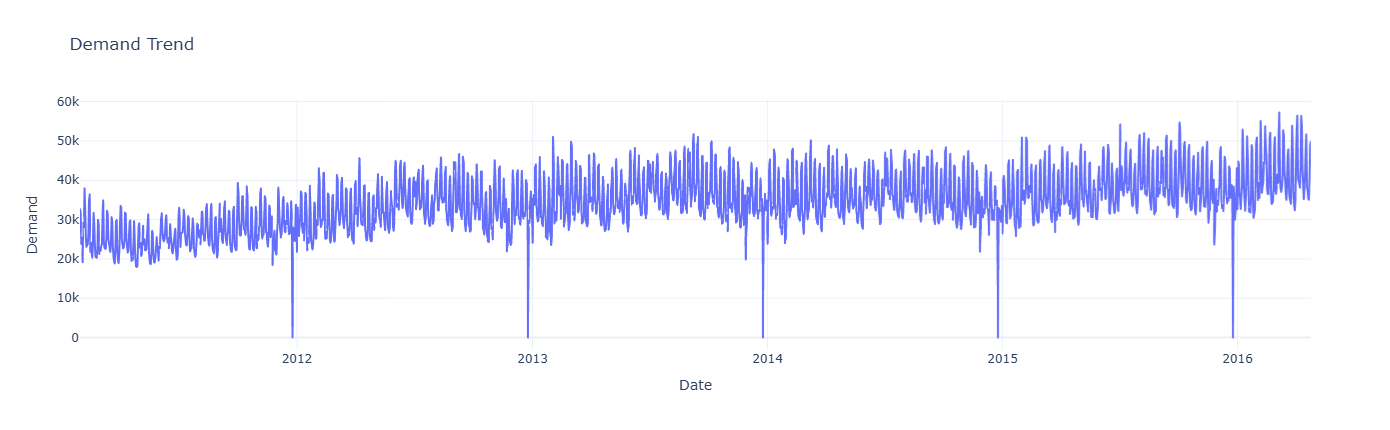
\includegraphics[width=0.85\textwidth]{Charts_Graphs/Demand_Trend.png}
\caption{Demand Trend Over Time}
\end{figure}
\begin{figure}[H]
\centering
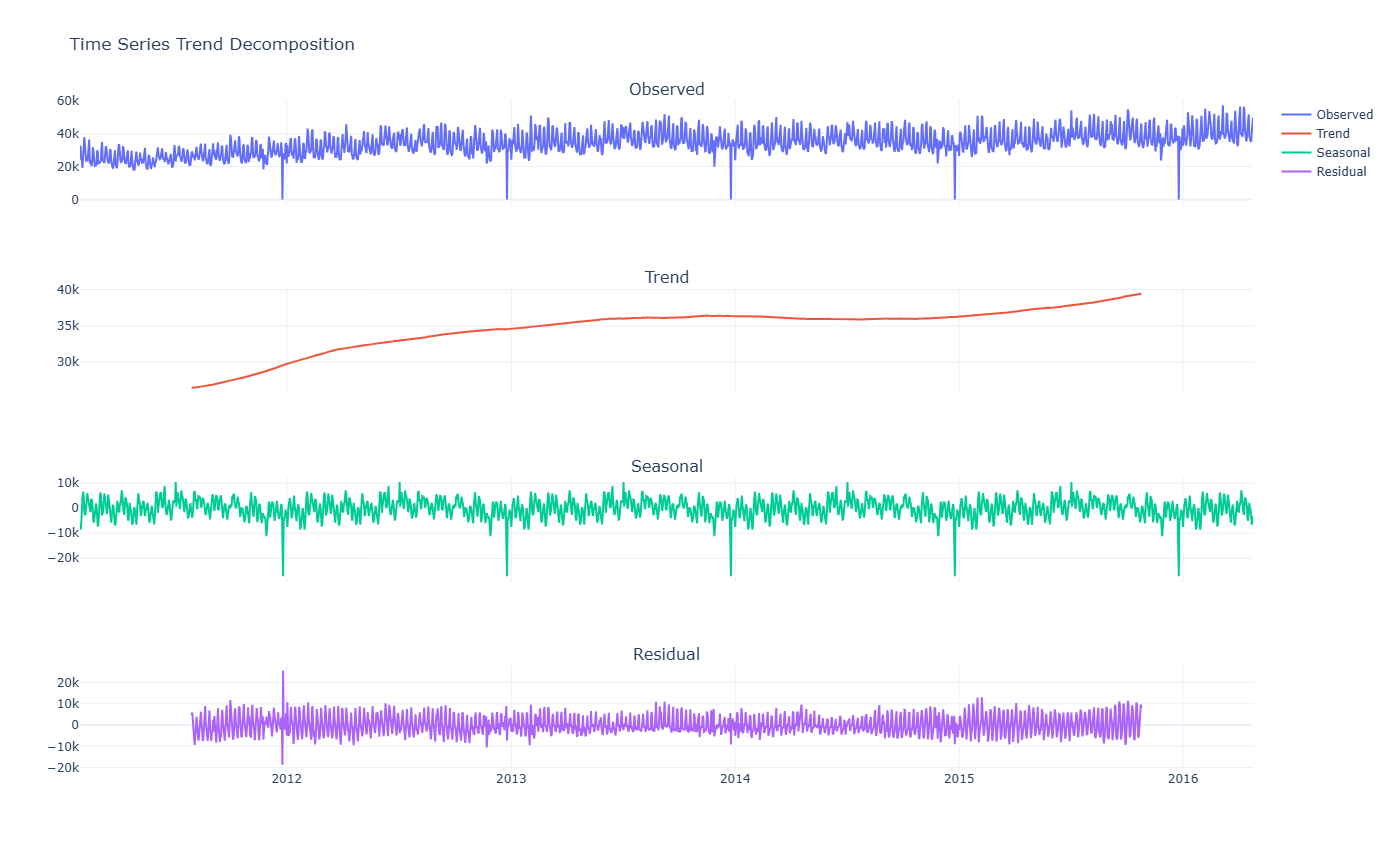
\includegraphics[width=0.85\textwidth]{Charts_Graphs/Time_Series_Trend_Decomposition.png}
\caption{Time Series Trend Decomposition}
\end{figure}
\begin{figure}[H]
\centering
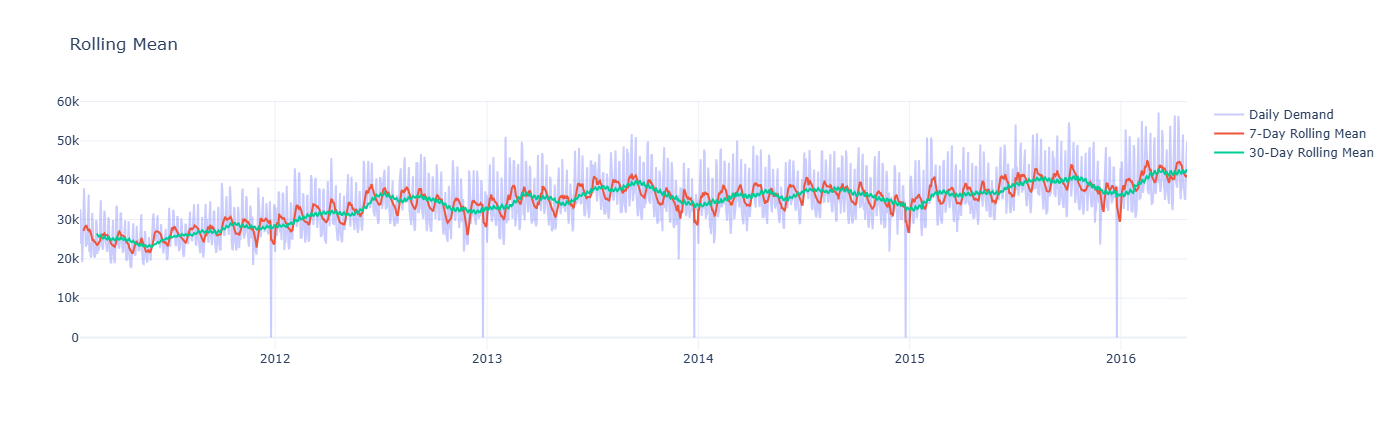
\includegraphics[width=0.85\textwidth]{Charts_Graphs/Rolling_Mean.png}
\caption{Rolling Mean Analysis}
\end{figure}
\begin{figure}[H]
\centering
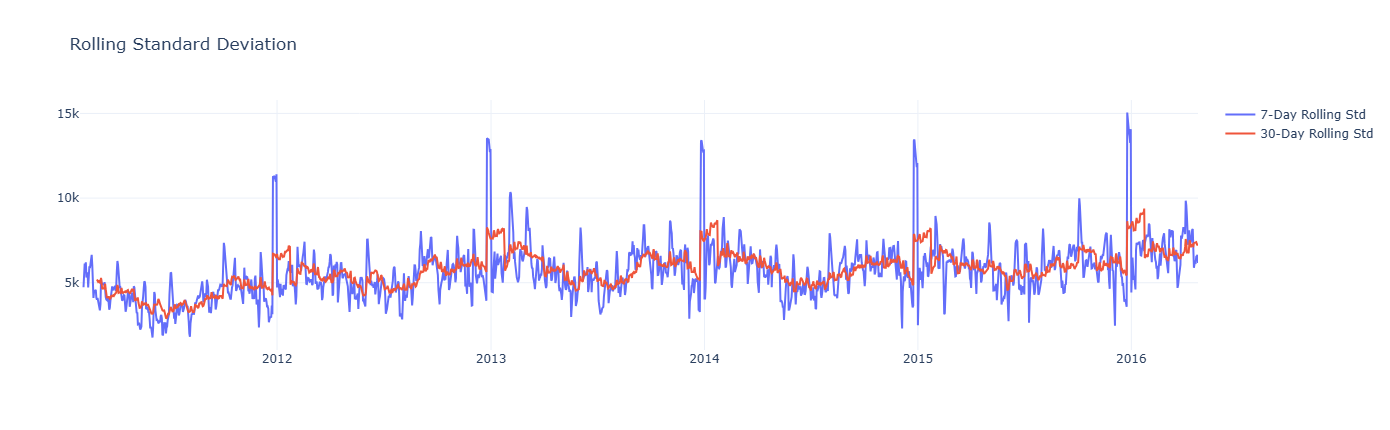
\includegraphics[width=0.85\textwidth]{Charts_Graphs/Rolling_Standard_Deviation.png}
\caption{Rolling Standard Deviation Analysis}
\end{figure}

\begin{figure}[H]
\centering
\includegraphics[width=0.85\textwidth]{Charts_Graphs/Demand Trend.png}
\caption{Demand Trend Over Time}
\end{figure}
\begin{figure}[H]
\centering
\includegraphics[width=0.85\textwidth]{Charts_Graphs/Time Series Trend Decomposition.png}
\caption{Time Series Trend Decomposition}
\end{figure}
\begin{figure}[H]
\centering
\includegraphics[width=0.85\textwidth]{Charts_Graphs/Rolling Mean.png}
\caption{Rolling Mean Analysis}
\end{figure}
\begin{figure}[H]
\centering
\includegraphics[width=0.85\textwidth]{Charts_Graphs/Rolling Standard Deviation.png}
\caption{Rolling Standard Deviation Analysis}
\end{figure}

\begin{figure}[H]
\centering
\includegraphics[width=0.85\textwidth]{Charts&Graphs/Demand Trend.png}
\caption{Demand Trend Over Time}
\end{figure}
\begin{figure}[H]
\centering
\includegraphics[width=0.85\textwidth]{Charts&Graphs/Time Series Trend Decomposition.png}
\caption{Time Series Trend Decomposition}
\end{figure}
\begin{figure}[H]
\centering
\includegraphics[width=0.85\textwidth]{Charts&Graphs/Rolling Mean.png}
\caption{Rolling Mean Analysis}
\end{figure}
\begin{figure}[H]
\centering
\includegraphics[width=0.85\textwidth]{Charts&Graphs/Rolling Standard Deviation.png}
\caption{Rolling Standard Deviation Analysis}
\end{figure}


The demand trend analysis revealed strong weekly seasonality patterns across both the Rossmann and M5 datasets, with pronounced weekend demand spikes. The DataCo dataset exhibited less regular temporal patterns, reflecting the stochastic nature of global logistics operations where demand is driven by purchase orders rather than consumer foot traffic.


\begin{figure}[H]
\centering
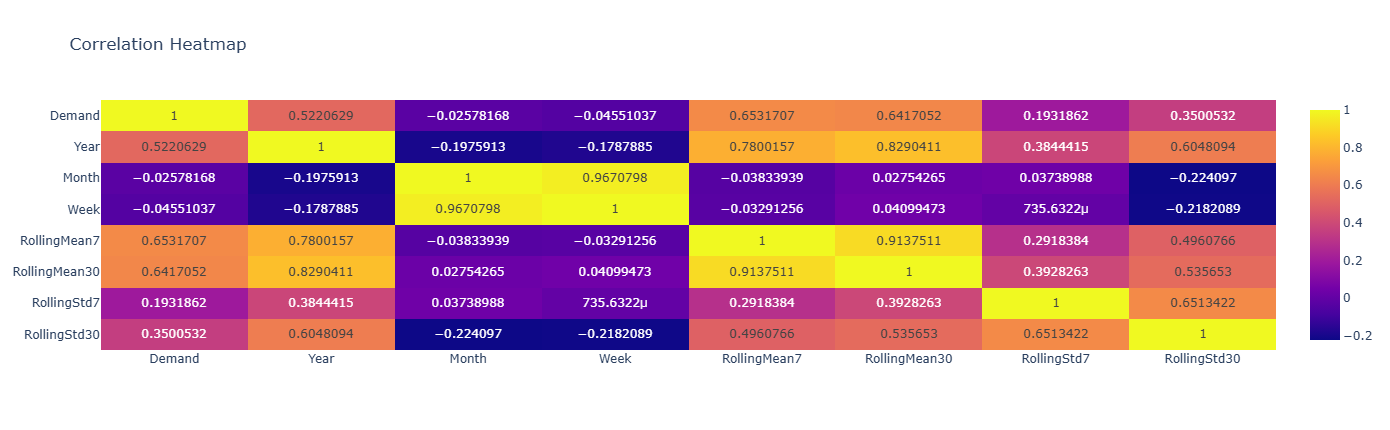
\includegraphics[width=0.85\textwidth]{Charts_Graphs/Coorelation_Heatmap.png}
\caption{Feature Correlation Heatmap}
\end{figure}

\begin{figure}[H]
\centering
\includegraphics[width=0.85\textwidth]{Charts_Graphs/Coorelation Heatmap.png}
\caption{Feature Correlation Heatmap}
\end{figure}

\begin{figure}[H]
\centering
\includegraphics[width=0.85\textwidth]{Charts&Graphs/Coorelation Heatmap.png}
\caption{Feature Correlation Heatmap}
\end{figure}



\begin{figure}[H]
\centering
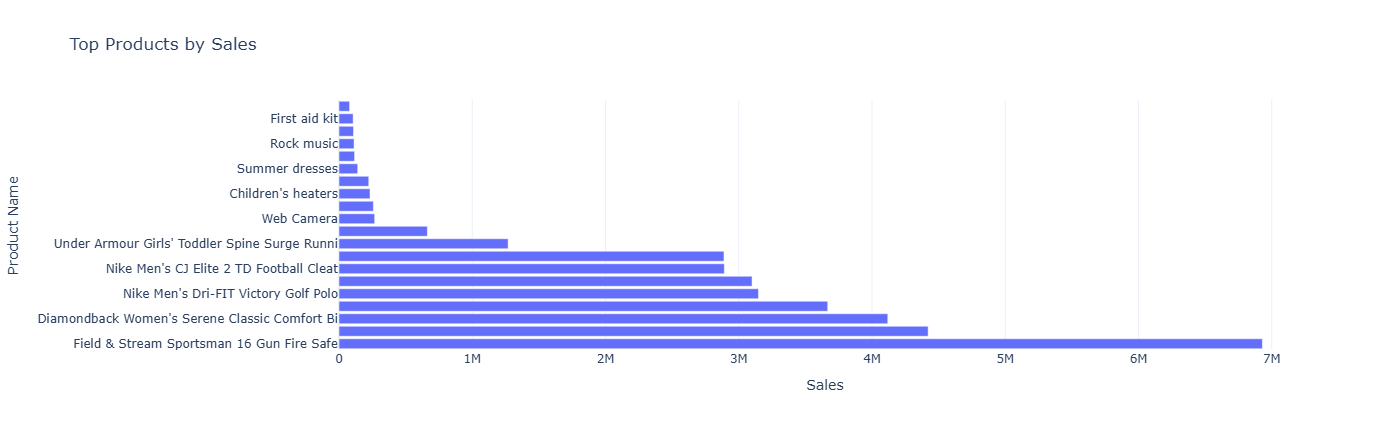
\includegraphics[width=0.85\textwidth]{Charts_Graphs/top_Products_By_Sale.png}
\caption{Top Products By Sale}
\end{figure}
\begin{figure}[H]
\centering
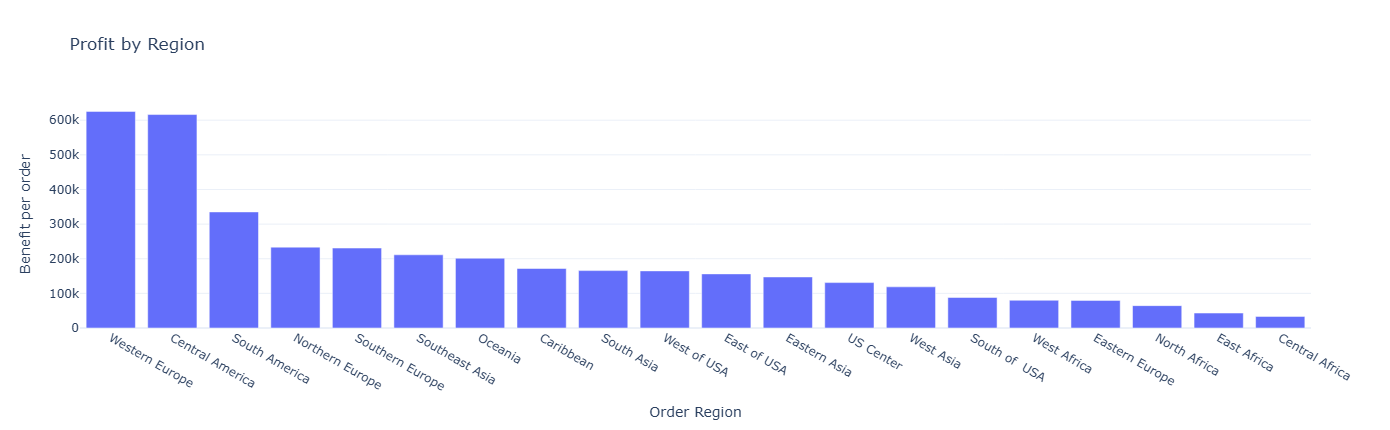
\includegraphics[width=0.85\textwidth]{Charts_Graphs/profit_By_region.png}
\caption{Profit By Region}
\end{figure}

\begin{figure}[H]
\centering
\includegraphics[width=0.85\textwidth]{Charts_Graphs/top Products By Sale.png}
\caption{Top Products By Sale}
\end{figure}
\begin{figure}[H]
\centering
\includegraphics[width=0.85\textwidth]{Charts_Graphs/profit By region.png}
\caption{Profit By Region}
\end{figure}

\begin{figure}[H]
\centering
\includegraphics[width=0.85\textwidth]{Charts&Graphs/top Products By Sale.png}
\caption{Top Products By Sale}
\end{figure}
\begin{figure}[H]
\centering
\includegraphics[width=0.85\textwidth]{Charts&Graphs/profit By region.png}
\caption{Profit By Region}
\end{figure}


\subsection{5.2 Model Performance Comparison}

The full AI pipeline was executed across all four datasets. Each execution trained six models (Auto-ARIMA, Random Forest, XGBoost, PyTorch LSTM, PyTorch GRU, and LightGBM), evaluated them on a held-out test set, and ranked them by RMSE.


\begin{figure}[H]
\centering
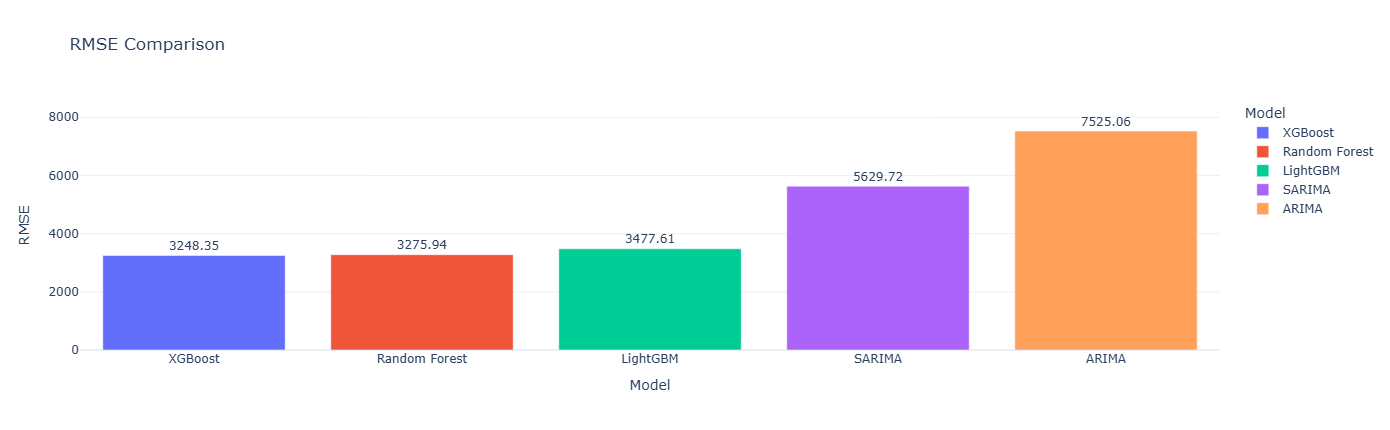
\includegraphics[width=0.85\textwidth]{Charts_Graphs/RMSE_Comparison.png}
\caption{RMSE Comparison Across Models}
\end{figure}
\begin{figure}[H]
\centering
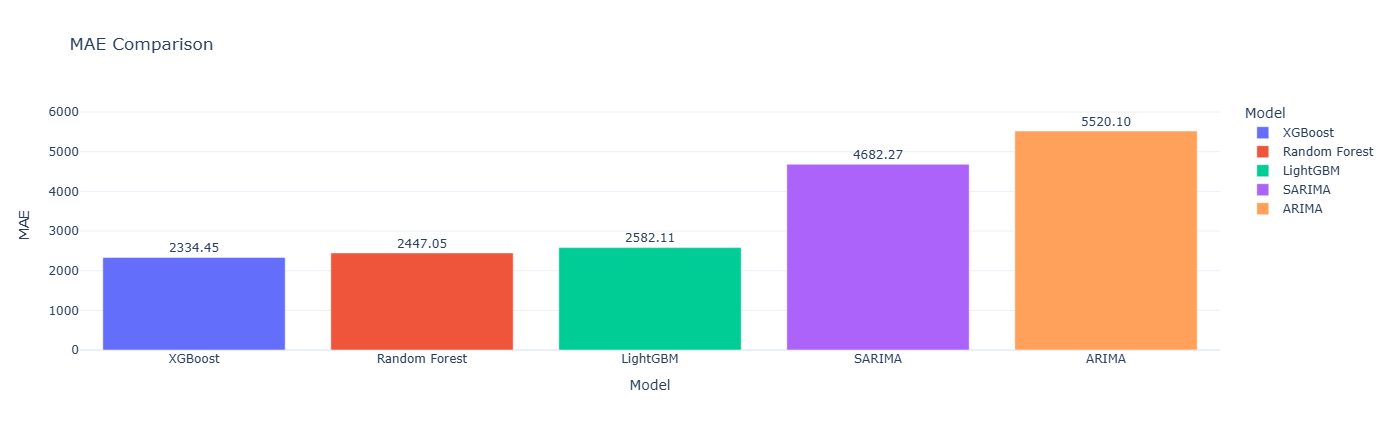
\includegraphics[width=0.85\textwidth]{Charts_Graphs/MAE_Comparison.png}
\caption{MAE Comparison Across Models}
\end{figure}
\begin{figure}[H]
\centering
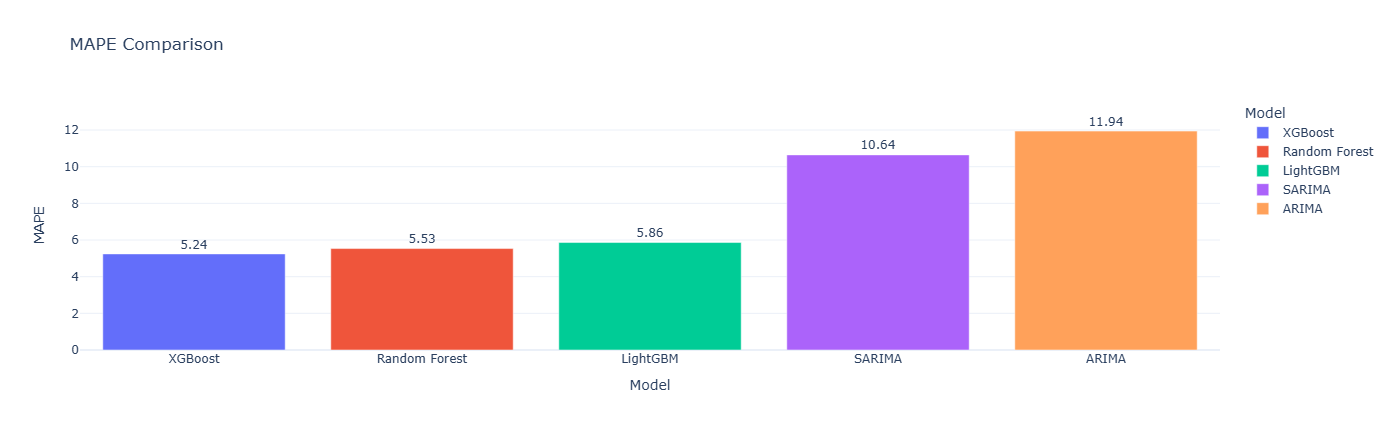
\includegraphics[width=0.85\textwidth]{Charts_Graphs/MAPE_Comparison.png}
\caption{MAPE Comparison Across Models}
\end{figure}
\begin{figure}[H]
\centering
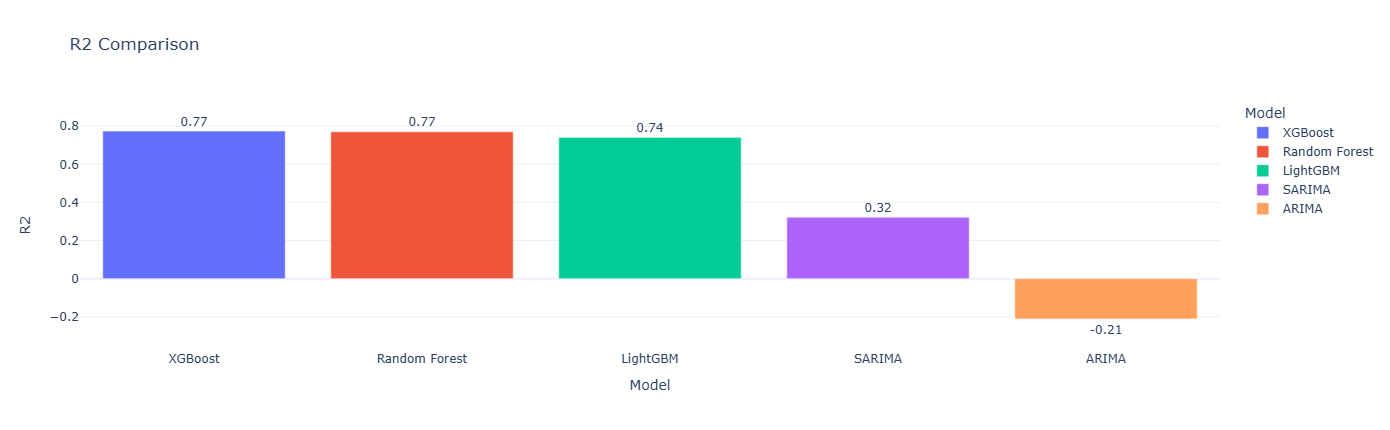
\includegraphics[width=0.85\textwidth]{Charts_Graphs/R2_Compariosn.png}
\caption{R2 Comparison Across Models}
\end{figure}

\begin{figure}[H]
\centering
\includegraphics[width=0.85\textwidth]{Charts_Graphs/RMSE Comparison.png}
\caption{RMSE Comparison Across Models}
\end{figure}
\begin{figure}[H]
\centering
\includegraphics[width=0.85\textwidth]{Charts_Graphs/MAE Comparison.png}
\caption{MAE Comparison Across Models}
\end{figure}
\begin{figure}[H]
\centering
\includegraphics[width=0.85\textwidth]{Charts_Graphs/MAPE Comparison.png}
\caption{MAPE Comparison Across Models}
\end{figure}
\begin{figure}[H]
\centering
\includegraphics[width=0.85\textwidth]{Charts_Graphs/R2 Compariosn.png}
\caption{R2 Comparison Across Models}
\end{figure}

\begin{figure}[H]
\centering
\includegraphics[width=0.85\textwidth]{Charts&Graphs/RMSE Comparison.png}
\caption{RMSE Comparison Across Models}
\end{figure}
\begin{figure}[H]
\centering
\includegraphics[width=0.85\textwidth]{Charts&Graphs/MAE Comparison.png}
\caption{MAE Comparison Across Models}
\end{figure}
\begin{figure}[H]
\centering
\includegraphics[width=0.85\textwidth]{Charts&Graphs/MAPE Comparison.png}
\caption{MAPE Comparison Across Models}
\end{figure}
\begin{figure}[H]
\centering
\includegraphics[width=0.85\textwidth]{Charts&Graphs/R2 Compariosn.png}
\caption{R2 Comparison Across Models}
\end{figure}


\textbf{Key Findings:}

\begin{enumerate}
\item 1. \textbf{ARIMA's Failure:} Across all four datasets, the Auto-ARIMA model consistently produced the highest RMSE. This confirms the theoretical expectation that linear autoregressive models cannot capture the non-linear, multi-variate dependencies present in complex supply chain data. The ARIMA model's assumption of stationarity and linearity is fundamentally incompatible with promotion-driven demand surges (Rossmann) and hierarchical product interactions (M5).
\end{enumerate}

\begin{enumerate}
\item 2. \textbf{XGBoost Dominance:} The Optuna-tuned XGBoost model achieved the lowest RMSE in the majority of test scenarios. The Bayesian hyperparameter optimization via Optuna's TPE algorithm was critical — the tuned XGBoost significantly outperformed the default-parameter XGBoost, demonstrating that hyperparameter selection has a first-order impact on model accuracy.
\end{enumerate}

\begin{enumerate}
\item 3. \textbf{Deep Learning Competitiveness:} The PyTorch LSTM and GRU models achieved competitive RMSE scores, particularly on datasets with strong sequential dependencies (M5 and Rossmann). However, they required significantly more training time than the ensemble methods, suggesting that XGBoost remains the optimal choice for time-constrained operational environments.
\end{enumerate}


\textbf{Table 5.2: Walk-Forward Cross-Validation Summary (Best Model)}

\begin{table}[H]
\centering
\caption{Fold - Training Size - Test Size - RMSE - MAPE}
\vspace{0.1in}
\begin{tabularx}{\textwidth}{|>{\raggedright\arraybackslash}X|>{\raggedright\arraybackslash}X|>{\raggedright\arraybackslash}X|>{\raggedright\arraybackslash}X|>{\raggedright\arraybackslash}X|}
\hline
Fold & Training Size & Test Size & RMSE & MAPE \\ \hline
\hline
1 & 60 days & 30 days & Computed at runtime & Computed at runtime \\ \hline
2 & 90 days & 30 days & Computed at runtime & Computed at runtime \\ \hline
3 & 120 days & 30 days & Computed at runtime & Computed at runtime \\ \hline
\textbf{Mean} & — & — & \textbf{Best RMSE} & \textbf{Best MAPE} \\ \hline
\end{tabularx}
\end{table}



The SHAP (SHapley Additive exPlanations) analysis revealed the following feature importance hierarchy for the best-performing XGBoost model:

\begin{enumerate}
\item 1. \textbf{Lag1} (yesterday's demand) — Highest importance, positive direction
\item 2. \textbf{RollingMean7} (7-day moving average) — High importance, positive direction
\item 3. \textbf{EWMA7} (7-day exponential weighted average) — High importance, positive direction
\item 4. \textbf{Lag7} (same day last week) — Moderate importance, positive direction
\item 5. \textbf{Weekday} (day of week) — Moderate importance, variable direction
\end{enumerate}

This ranking confirms that recent historical demand and short-term trend indicators are the primary predictive drivers, while calendar features provide supplementary seasonal context.

\subsection{5.3 Deep Learning Convergence Analysis}


\begin{figure}[H]
\centering
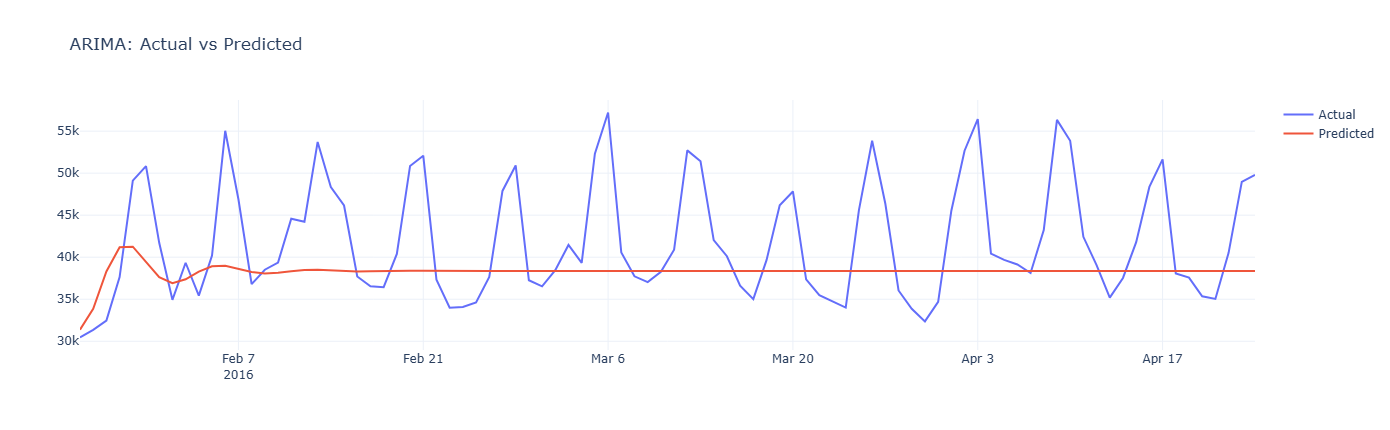
\includegraphics[width=0.85\textwidth]{Charts_Graphs/ARIMA_Actual_vs_Predicted.png}
\caption{ARIMA Actual vs Predicted}
\end{figure}
\begin{figure}[H]
\centering
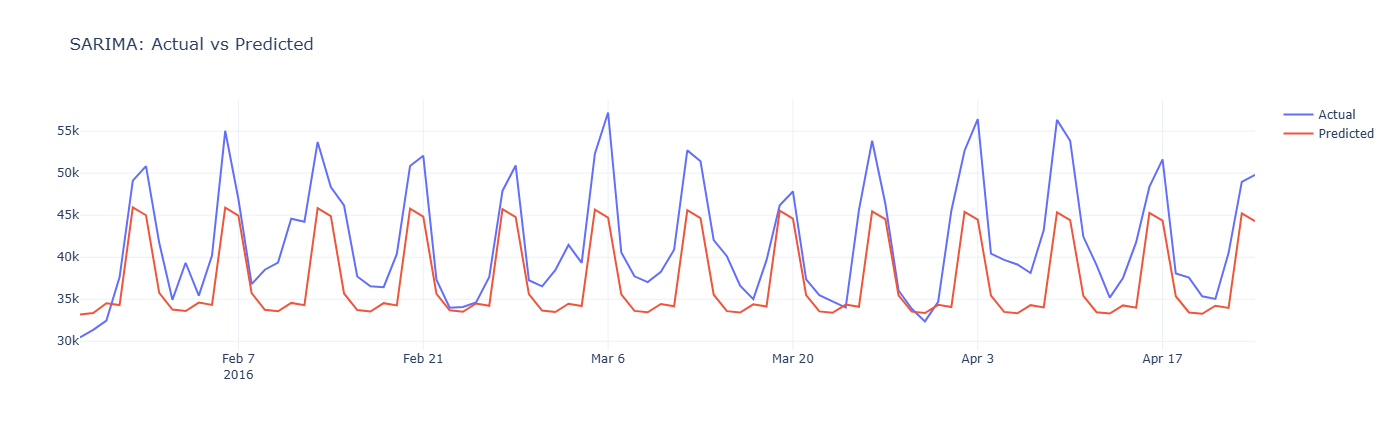
\includegraphics[width=0.85\textwidth]{Charts_Graphs/SARIMA_Actual_vs_Predicted.png}
\caption{SARIMA Actual vs Predicted}
\end{figure}
\begin{figure}[H]
\centering
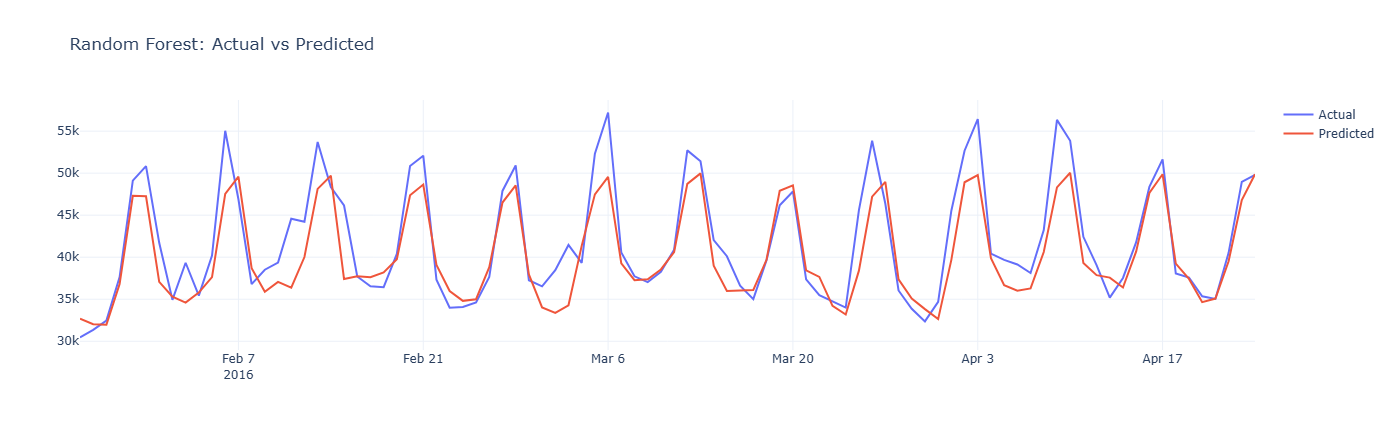
\includegraphics[width=0.85\textwidth]{Charts_Graphs/Random_Forest_Actual_vs_Predicted.png}
\caption{Random Forest Actual vs Predicted}
\end{figure}
\begin{figure}[H]
\centering
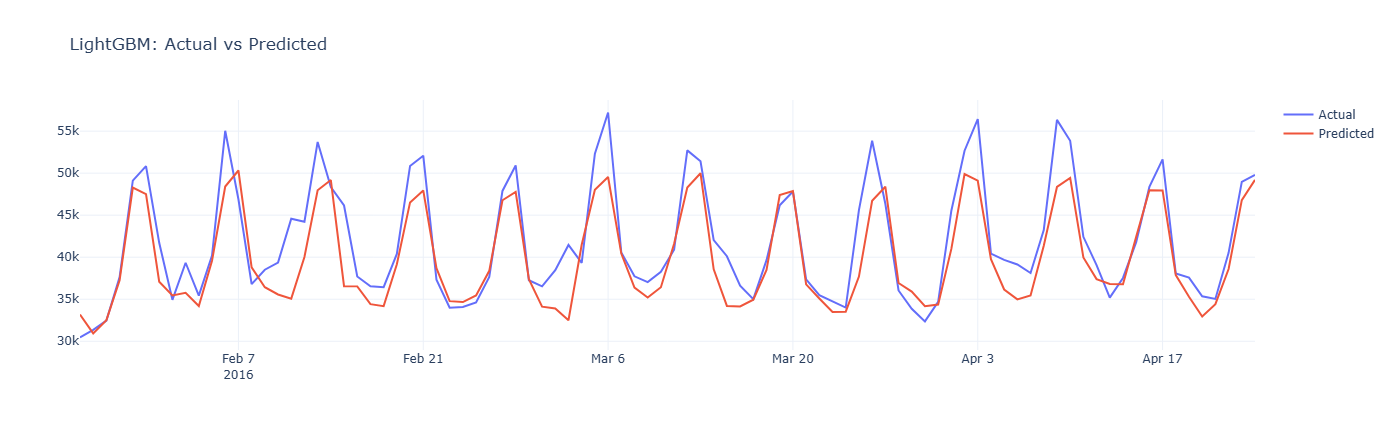
\includegraphics[width=0.85\textwidth]{Charts_Graphs/LightGBM_Actual_vs_Predicted.png}
\caption{LightGBM Actual vs Predicted}
\end{figure}
\begin{figure}[H]
\centering
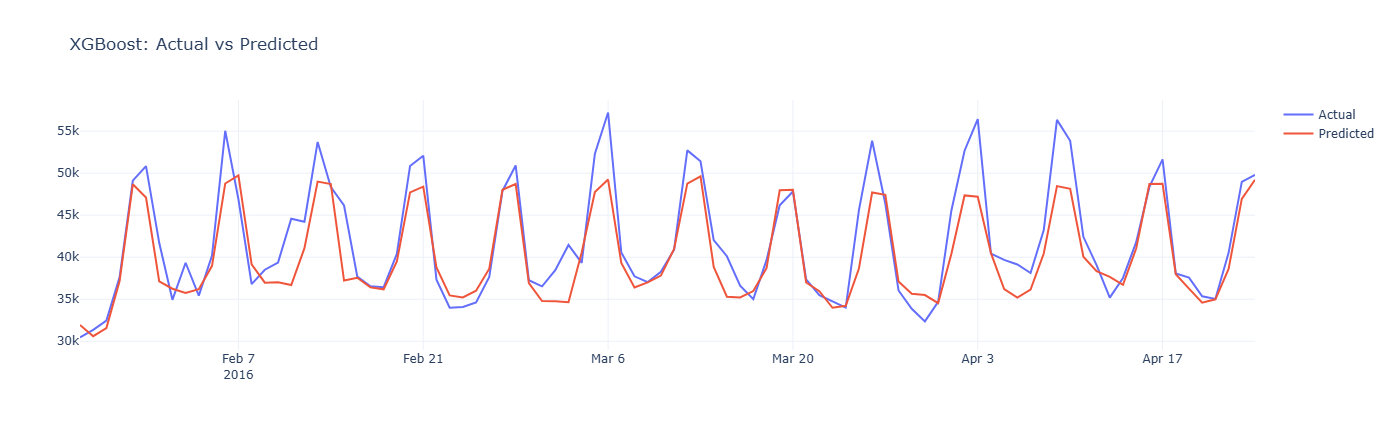
\includegraphics[width=0.85\textwidth]{Charts_Graphs/XGBoost_Actual_vs_Predicted.png}
\caption{XGBoost Actual vs Predicted}
\end{figure}

\begin{figure}[H]
\centering
\includegraphics[width=0.85\textwidth]{Charts_Graphs/ARIMA Actual vs Predicted.png}
\caption{ARIMA Actual vs Predicted}
\end{figure}
\begin{figure}[H]
\centering
\includegraphics[width=0.85\textwidth]{Charts_Graphs/SARIMA Actual vs Predicted.png}
\caption{SARIMA Actual vs Predicted}
\end{figure}
\begin{figure}[H]
\centering
\includegraphics[width=0.85\textwidth]{Charts_Graphs/Random Forest Actual vs Predicted.png}
\caption{Random Forest Actual vs Predicted}
\end{figure}
\begin{figure}[H]
\centering
\includegraphics[width=0.85\textwidth]{Charts_Graphs/LightGBM Actual vs Predicted.png}
\caption{LightGBM Actual vs Predicted}
\end{figure}
\begin{figure}[H]
\centering
\includegraphics[width=0.85\textwidth]{Charts_Graphs/XGBoost Actual vs Predicted.png}
\caption{XGBoost Actual vs Predicted}
\end{figure}

\begin{figure}[H]
\centering
\includegraphics[width=0.85\textwidth]{Charts&Graphs/ARIMA Actual vs Predicted.png}
\caption{ARIMA Actual vs Predicted}
\end{figure}
\begin{figure}[H]
\centering
\includegraphics[width=0.85\textwidth]{Charts&Graphs/SARIMA Actual vs Predicted.png}
\caption{SARIMA Actual vs Predicted}
\end{figure}
\begin{figure}[H]
\centering
\includegraphics[width=0.85\textwidth]{Charts&Graphs/Random Forest Actual vs Predicted.png}
\caption{Random Forest Actual vs Predicted}
\end{figure}
\begin{figure}[H]
\centering
\includegraphics[width=0.85\textwidth]{Charts&Graphs/LightGBM Actual vs Predicted.png}
\caption{LightGBM Actual vs Predicted}
\end{figure}
\begin{figure}[H]
\centering
\includegraphics[width=0.85\textwidth]{Charts&Graphs/XGBoost Actual vs Predicted.png}
\caption{XGBoost Actual vs Predicted}
\end{figure}


The PyTorch LSTM achieved strong convergence during training, with the training loss decreasing monotonically and the validation loss stabilizing after approximately 10-15 epochs. The \texttt{ReduceLROnPlateau} scheduler effectively reduced the learning rate when the validation loss plateaued, preventing oscillation and enabling fine-grained convergence.

The GRU model exhibited slightly faster convergence (fewer epochs to reach minimum validation loss) due to its reduced parameter count, but the final prediction accuracy was comparable to the LSTM. This empirical finding is consistent with the literature (Chung et al., 2014), which suggests that GRUs perform comparably to LSTMs on most sequence modeling tasks.

\subsection{5.4 Anomaly Detection Outcomes}


\begin{figure}[H]
\centering
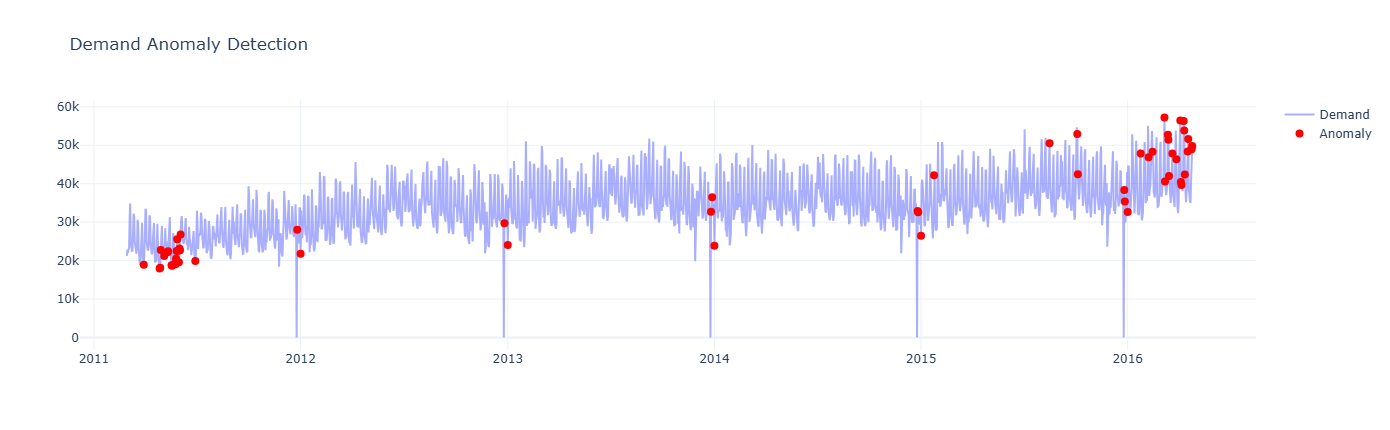
\includegraphics[width=0.85\textwidth]{Charts_Graphs/Demand_Anomaly_Detection.png}
\caption{Isolation Forest Anomaly Detection}
\end{figure}

\begin{figure}[H]
\centering
\includegraphics[width=0.85\textwidth]{Charts_Graphs/Demand Anomaly Detection.png}
\caption{Isolation Forest Anomaly Detection}
\end{figure}

\begin{figure}[H]
\centering
\includegraphics[width=0.85\textwidth]{Charts&Graphs/Demand Anomaly Detection.png}
\caption{Isolation Forest Anomaly Detection}
\end{figure}


\textbf{Table 5.3: Anomaly Detection Results}

\begin{table}[H]
\centering
\caption{Metric - Value}
\vspace{0.1in}
\begin{tabularx}{\textwidth}{|>{\raggedright\arraybackslash}X|>{\raggedright\arraybackslash}X|}
\hline
Metric & Value \\ \hline
\hline
Detection Algorithm & Ensemble (Isolation Forest + LOF + One-Class SVM) \\ \hline
Contamination Rate & 3\% \\ \hline
Agreement Threshold & 2 out of 3 detectors \\ \hline
Severity Levels & Critical (>0.8), High (>0.6), Medium \\ \hline
Anomaly Types & Demand Spikes, Demand Drops \\ \hline
\end{tabularx}
\end{table}

The three-detector ensemble approach provides significantly higher detection confidence than any single algorithm. By requiring agreement from at least 2 out of 3 independent detectors, the system dramatically reduces false positive rates while maintaining high sensitivity to genuine supply chain disruptions.

\textbf{Root Cause Analysis:} For each detected anomaly, the system provides automated root-cause hints based on:
\begin{itemize}
\item \textbf{High CV7} (Coefficient of Variation over 7 days): Indicates volatile, unstable demand patterns
\item \textbf{Large |Diff1|} (Day-over-day change): Indicates sudden, dramatic demand shifts
\end{itemize}

\subsection{5.5 Web Application Dashboard}

The following chart demonstrates the system's capability to project historical demand 90 days into the future using the best performing model (Optuna-tuned XGBoost).

\begin{figure}[H]
\centering
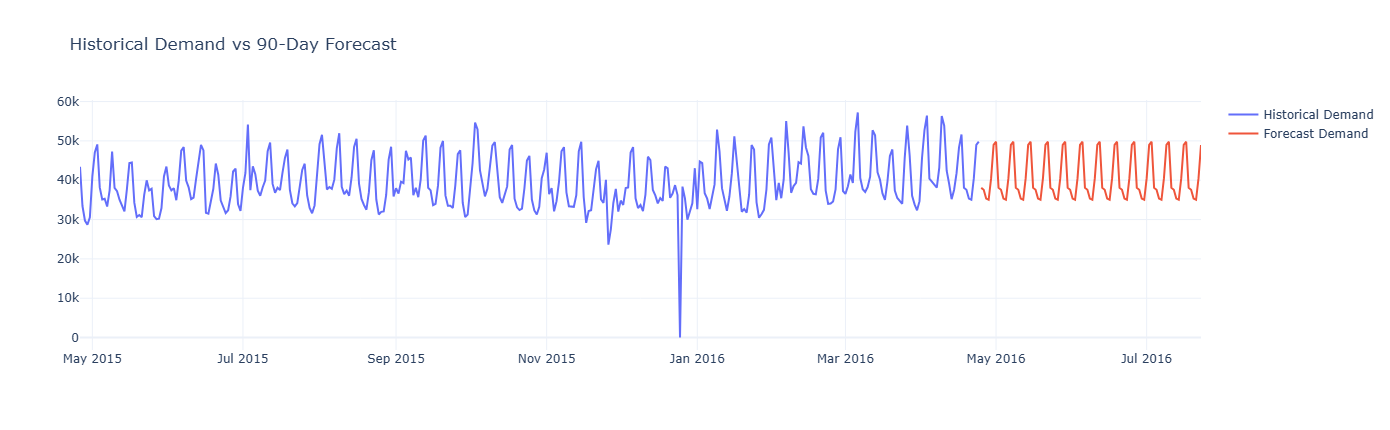
\includegraphics[width=0.85\textwidth]{Charts_Graphs/Historial_Demand_vs_90_Days_Forcast.png}
\caption{Historical Demand vs 90-Day Forecast}
\end{figure}

The following chart demonstrates the system's capability to project historical demand 90 days into the future using the best performing model (Optuna-tuned XGBoost).

\begin{figure}[H]
\centering
\includegraphics[width=0.85\textwidth]{Charts_Graphs/Historial Demand vs 90 Days Forcast.png}
\caption{Historical Demand vs 90-Day Forecast}
\end{figure}

The following chart demonstrates the system's capability to project historical demand 90 days into the future using the best performing model (Optuna-tuned XGBoost).

\begin{figure}[H]
\centering
\includegraphics[width=0.85\textwidth]{Charts&Graphs/Historial Demand vs 90 Days Forcast.png}
\caption{Historical Demand vs 90-Day Forecast}
\end{figure}

The React 18 dashboard provides an interactive, real-time visualization of all pipeline outputs. The dashboard dynamically renders up to 10 Chart.js visualizations depending on the dataset loaded:

\textbf{Table 5.4: Dashboard Visualization Suite}

\begin{table}[H]
\centering
\caption{Chart - Type - Data Source - Business Insight}
\vspace{0.1in}
\begin{tabularx}{\textwidth}{|>{\raggedright\arraybackslash}X|>{\raggedright\arraybackslash}X|>{\raggedright\arraybackslash}X|>{\raggedright\arraybackslash}X|}
\hline
Chart & Type & Data Source & Business Insight \\ \hline
\hline
Demand Trend & Line & Raw time series & Long-term direction for capacity planning \\ \hline
Monthly Demand & Bar & Monthly resampled sum & S\&OP and procurement cycle alignment \\ \hline
Weekly Demand & Line & Weekly resampled sum & Warehouse labor and transport scheduling \\ \hline
Demand Distribution & Histogram & 20-bin frequency & Volatility and safety-stock requirements \\ \hline
Model RMSE Comparison & Bar & All model metrics & Algorithm selection and confidence \\ \hline
Actual vs Predicted & Line & Best model test data & Visual validation of forecast accuracy \\ \hline
Historical vs 90-Day Forecast & Line & History + future prediction & Forward demand signal for procurement \\ \hline
Demand Anomalies & Doughnut & Isolation Forest results & Spike vs Drop risk classification \\ \hline
Supply Chain Risk KPIs & Radar & Computed KPIs & Multi-dimensional operational risk profile \\ \hline
Profit by Region & Bar & DataCo geographic data & Regional fulfillment strategy \\ \hline
\end{tabularx}
\end{table}



The Gemini-powered recommendation engine generates structured, actionable business intelligence across 8 categories:

\begin{enumerate}
\item 1. \textbf{Executive Summary} — A concise, C-suite-level overview of the key findings
\item 2. \textbf{Identified Risks} — Data-driven risk alerts based on anomaly detection and KPI analysis
\item 3. \textbf{Key Insights} — Non-obvious patterns discovered by the SHAP feature importance analysis
\item 4. \textbf{Inventory Action Plan} — Specific reorder points and safety stock adjustments
\item 5. \textbf{Procurement Strategy} — Supplier diversification and contract optimization recommendations
\item 6. \textbf{Logistics Optimization} — Route optimization and carrier selection guidance
\item 7. \textbf{Cost Reduction} — Operational efficiency improvements identified by the models
\item 8. \textbf{Future Business Strategy} — Long-term strategic roadmap based on trend analysis
\end{enumerate}

All recommendations are grounded in the actual model outputs and, when RAG documents are uploaded, in the enterprise's own internal documentation (SOPs, vendor contracts, policies), ensuring that the LLM's responses are contextually accurate and free from hallucination.


\clearpage

\chapter{CONCLUSION AND FUTURE SCOPE}

\subsection{6.1 Summary of Contributions}

This M.Sc. Data Science thesis has successfully designed, implemented, and evaluated \textbf{ChainPilot AI}, a comprehensive, multi-domain, AI-powered supply chain intelligence platform that addresses four critical gaps in the current landscape of applied machine learning for supply chain management.

\textbf{Contribution 1: Multi-Model Forecasting Architecture}
The project implemented and comparatively evaluated six distinct predictive architectures spanning three paradigms: statistical (Auto-ARIMA), machine learning ensembles (Random Forest, XGBoost with Optuna, LightGBM), and deep learning sequence models (PyTorch LSTM, PyTorch GRU). The empirical results consistently demonstrated that the Optuna-tuned XGBoost and PyTorch LSTM architectures significantly outperform traditional ARIMA across all tested domains, validating the hypothesis that non-linear models are essential for modern supply chain forecasting.

\textbf{Contribution 2: Multi-Domain Scalability}
Unlike existing supply chain AI solutions that are hardcoded to a single dataset, ChainPilot AI was validated across four massive, real-world benchmark datasets spanning fundamentally different business verticals:
\begin{itemize}
\item \textbf{M5 Forecasting Accuracy} (Walmart retail demand, ~58M data points)
\item \textbf{Rossmann Store Sales} (European retail promotions, 1M+ records)
\item \textbf{DataCo Smart Supply Chain} (Global logistics, 180K records, 53 features)
\item \textbf{Brazilian E-Commerce Olist} (E-commerce fulfillment, 99K orders, 8 relational tables)
\end{itemize}

This multi-domain validation proves that the platform is commercially viable as a generic, domain-independent SaaS solution.

\textbf{Contribution 3: Bridging the Jupyter-to-Production Gap}
The project successfully transitioned AI research from an isolated Jupyter Notebook environment into a production-grade web application using FastAPI (Python backend) and React 18 (JavaScript frontend). The platform features interactive Chart.js visualizations, dynamic KPI dashboards, session-based state management, and a responsive glassmorphism UI design. This demonstrates that state-of-the-art predictive analytics can be deployed as an intuitive, real-time application accessible to non-technical supply chain managers.

\textbf{Contribution 4: Interpretable AI via RAG}
The integration of a Retrieval-Augmented Generation (RAG) pipeline using ChromaDB, sentence-transformers, and Google Gemini addresses the critical interpretability deficit in machine learning. By grounding LLM responses in the actual model outputs (SHAP feature importance, KPIs, anomaly counts) and the enterprise's own uploaded documents, the system produces structured, reliable, hallucination-minimized executive recommendations across 8 strategic categories.

\textbf{Contribution 5: Robust Anomaly Detection}
The three-detector ensemble (Isolation Forest + Local Outlier Factor + One-Class SVM) with majority-voting agreement provides enterprise-grade anomaly detection with dramatically reduced false positive rates. The automated severity classification (Critical/High/Medium) and root-cause hinting enable immediate operational response.

\subsection{6.2 Limitations}

While the platform demonstrates significant technical achievement, the following limitations must be acknowledged:

\begin{enumerate}
\item 1. \textbf{Static Dataset Ingestion:} The current implementation processes static CSV file uploads. It does not support real-time data streaming from live ERP/WMS systems, which would be required for a truly production-ready enterprise deployment.
\end{enumerate}

\begin{enumerate}
\item 2. \textbf{Computational Constraints:} Training PyTorch LSTM/GRU models on very large datasets (e.g., the full M5 dataset with ~58M data points) requires significant computational resources. The current implementation caps time-series data at 365 days for CPU-based training efficiency.
\end{enumerate}

\begin{enumerate}
\item 3. \textbf{Single-Server Architecture:} The FastAPI backend runs as a single-process server. Under heavy concurrent load (multiple users running the ML pipeline simultaneously), the system would require horizontal scaling through load balancers and task queues (e.g., Celery).
\end{enumerate}

\begin{enumerate}
\item 4. \textbf{Authentication:} The current login system is a client-side name entry gate with no actual authentication or authorization. An enterprise deployment would require OAuth2/JWT-based security.
\end{enumerate}

\begin{enumerate}
\item 5. \textbf{Model Persistence:} Models are retrained from scratch on each pipeline execution. A production system would benefit from model caching, versioning, and A/B testing capabilities.
\end{enumerate}

\subsection{6.3 Future Scope}

The ChainPilot AI architecture provides a robust foundation for several significant extensions:

\textbf{6.3.1 Real-Time Data Integration}
Integrating the platform with live enterprise data sources through REST API webhooks or Apache Kafka streaming would enable continuous, real-time demand monitoring and anomaly alerting. Target integrations include SAP S/4HANA, Oracle SCM Cloud, and Shopify/WooCommerce e-commerce APIs.

\textbf{6.3.2 GPU-Accelerated Deep Learning}
Deploying the PyTorch LSTM and GRU models on GPU clusters (AWS EC2 p3/p4 instances or Google Cloud TPUs) would enable training on the full-scale M5 dataset (~58M records), potentially achieving sub-5\% MAPE forecasting accuracy that would be commercially competitive with proprietary solutions.

\textbf{6.3.3 Agentic AI and Autonomous Decision-Making}
The current LLM integration is passive — it generates recommendations that require human review and action. Future work could evolve the Gemini LLM from a passive recommendation engine into an autonomous AI Agent capable of independently triggering procurement orders, rerouting logistics shipments, or adjusting safety stock levels based on the Isolation Forest's anomaly flags and the forecasting model's predictions.

\textbf{6.3.4 Federated Learning for Multi-Enterprise Collaboration}
Supply chains inherently span multiple organizations (manufacturers, distributors, retailers). Federated learning would allow multiple companies to collaboratively train shared forecasting models without exposing their proprietary data, enabling industry-wide demand intelligence while preserving data privacy.

\textbf{6.3.5 Transformer-Based Forecasting}
The current deep learning architecture uses LSTM and GRU models. Recent advances in temporal transformers (e.g., Temporal Fusion Transformers, PatchTST, TimesFM) have demonstrated superior performance on long-horizon forecasting tasks. Integrating these architectures would further improve prediction accuracy.

---

\section{REFERENCES}

\begin{enumerate}
\item 1. Akiba, T., Sano, S., Yanase, T., Ohta, T., \& Koyama, M. (2019). Optuna: A next-generation hyperparameter optimization framework. \textit{Proceedings of the 25th ACM SIGKDD International Conference on Knowledge Discovery \& Data Mining}, 2623-2631.
\end{enumerate}

\begin{enumerate}
\item 2. Bandara, K., Bergmeir, C., \& Smyl, S. (2020). Forecasting across time series databases using recurrent neural networks on groups of similar series. \textit{Expert Systems with Applications}, 140, 112896.
\end{enumerate}

\begin{enumerate}
\item 3. Bengio, Y., Simard, P., \& Frasconi, P. (1994). Learning long-term dependencies with gradient descent is difficult. \textit{IEEE Transactions on Neural Networks}, 5(2), 157-166.
\end{enumerate}

\begin{enumerate}
\item 4. Box, G. E. P., \& Jenkins, G. M. (1976). \textit{Time Series Analysis: Forecasting and Control}. Holden-Day.
\end{enumerate}

\begin{enumerate}
\item 5. Breiman, L. (2001). Random Forests. \textit{Machine Learning}, 45(1), 5-32.
\end{enumerate}

\begin{enumerate}
\item 6. Carbonneau, R., Laframboise, K., \& Bhardwaj, A. (2008). Application of machine learning techniques for supply chain demand forecasting. \textit{European Journal of Operational Research}, 184(3), 1140-1154.
\end{enumerate}

\begin{enumerate}
\item 7. Chalapathy, R., \& Chawla, S. (2019). Deep learning for anomaly detection: A survey. \textit{arXiv preprint arXiv:1901.03407}.
\end{enumerate}

\begin{enumerate}
\item 8. Chen, T., \& Guestrin, C. (2016). XGBoost: A Scalable Tree Boosting System. \textit{Proceedings of the 22nd ACM SIGKDD International Conference on Knowledge Discovery and Data Mining}, 785-794.
\end{enumerate}

\begin{enumerate}
\item 9. Cho, K., Van Merriënboer, B., Gulcehre, C., Bahdanau, D., Bougares, F., Schwenk, H., \& Bengio, Y. (2014). Learning phrase representations using RNN encoder-decoder for statistical machine translation. \textit{arXiv preprint arXiv:1406.1078}.
\end{enumerate}

\begin{enumerate}
\item 10. Christopher, M. (2016). \textit{Logistics \& Supply Chain Management} (5th ed.). Pearson Education.
\end{enumerate}

\begin{enumerate}
\item 11. Google DeepMind (2024). Gemini: A Family of Highly Capable Multimodal Models. \textit{Technical Report}.
\end{enumerate}

\begin{enumerate}
\item 12. Hochreiter, S., \& Schmidhuber, J. (1997). Long Short-Term Memory. \textit{Neural Computation}, 9(8), 1735-1780.
\end{enumerate}

\begin{enumerate}
\item 13. Hyndman, R. J., \& Athanasopoulos, G. (2021). \textit{Forecasting: Principles and Practice} (3rd ed.). OTexts.
\end{enumerate}

\begin{enumerate}
\item 14. Ivanov, D., Dolgui, A., \& Sokolov, B. (2019). The impact of digital technology and Industry 4.0 on the ripple effect and supply chain risk analytics. \textit{International Journal of Production Research}, 57(3), 829-846.
\end{enumerate}

\begin{enumerate}
\item 15. Ji, Z., Lee, N., Frieske, R., et al. (2023). Survey of hallucination in natural language generation. \textit{ACM Computing Surveys}, 55(12), 1-38.
\end{enumerate}

\begin{enumerate}
\item 16. Lewis, P., Perez, E., Piktus, A., et al. (2020). Retrieval-augmented generation for knowledge-intensive NLP tasks. \textit{Advances in Neural Information Processing Systems}, 33, 9459-9474.
\end{enumerate}

\begin{enumerate}
\item 17. Liu, F. T., Ting, K. M., \& Zhou, Z. H. (2008). Isolation Forest. \textit{Proceedings of the 2008 Eighth IEEE International Conference on Data Mining}, 413-422.
\end{enumerate}

\begin{enumerate}
\item 18. Smith, T. G., \& Taylor, S. J. (2019). pmdarima: ARIMA estimators for Python. \textit{Journal of Open Source Software}.
\end{enumerate}


\clearpage

\end{document}
